\documentclass[11pt,a4paper]{article}
\usepackage[T1]{fontenc}
\usepackage[utf8]{inputenc}
\usepackage{amsmath,amssymb}
\usepackage{graphicx}
\usepackage{booktabs}
\usepackage{array}
\usepackage{siunitx}
\usepackage{enumitem}
\usepackage[margin=1in]{geometry}
\usepackage{caption}
\usepackage{float}
\usepackage[hidelinks]{hyperref}
\usepackage[table]{xcolor}
\usepackage{microtype}

\graphicspath{{figures/}}
\newcommand{\keff}{\kappa_{\mathrm{eff}}}
\newcommand{\pcm}{\,\mathrm{pcm}}
\newcommand{\doi}[1]{\,\href{https://doi.org/#1}{doi:#1}}
\renewcommand{\arraystretch}{1.25}
\setlength{\emergencystretch}{2.5em}

\title{\bf A finite-sector diffusion closure of the phase space nodal method:
formulation, implementation and test problems}

\author{
  Yuchao Xu \\
  \textit{University of South China}, China \\
  \texttt{yxu40@hotmail.com} \\
  \texttt{https://openpsn-ai.com}
}

\date{November 2026\\[2pt]
  \small Preprint. Companion to the OpenPSN framework paper \cite{openpsn2026};
  code: \texttt{github.com/xycjscs/OpenPSN}, branch \texttt{psn-4}.}

% Generated by scripts.study4_closure_report.
\newcommand{\StudyFourPairs}{434}
\newcommand{\StudyFourSmaller}{416}
\newcommand{\StudyFourMedianRatio}{0.437}
\newcommand{\StudyFourSignChanges}{39}

\begin{document}
\maketitle

\begin{abstract}
The phase space nodal method (PSN) \cite{psn2027} partitions phase space into
spatial nodes and finite angular cells and solves a diffusion-type equation in
each cell. The published error survey of the method, reproduced in the companion
OpenPSN paper \cite{openpsn2026}, shows eigenvalue errors that change sign along
a diagonal valley of the square checkerboard, with the crossing point moving as
the spatial subdivision changes. This paper formulates and assesses a closure in
which the face and vacuum terms are taken from the same weak form as the body
term, the diffusion tensor of each finite angular cell being the exact second
moment of the directions retained in that cell, including its $xy$ component.
The reduction is carried out direction by direction in one closure and per finite
angular cell in the other, with optional local azimuthal modes, so the discrete
unknowns stay attached to finite sectors rather than to a truncated angular
expansion. Both carry $A{+}1$ angular unknowns per sector at azimuthal degree $A$, so
they can be differenced point by point, and the direction-wise closure is the one
reported as the closure of record. Two algebraic identities are verified symbolically
--- the exact elimination of the nodal interior, and the impossibility of exact angular
transfer through a finite closure --- and the discretisation is checked against an
analytic vacuum-slab solution, against 14 exact rational and symbolic checks, and on
1002 measured grid points --- 130 checkerboard points of the cell-average closure, 314
checkerboard points of the direction-wise one, 384 points of the archived
single-assembly $S\times M$ sweep, 30 points of the C5G7 rectangular quarter core and
144 further assembly points of the direction-wise re-sweep. The direction-wise
checkerboard sweep has 279 negative differences and 35 positive ones in a single
azimuthal column. Of the 280 spatial refinements, 246 move the error toward zero and
the other 34 belong to that column. An additional 240 measurements at the benchmark
default $A{=}3$ yield negative differences throughout, with reductions in magnitude at
228 of 228 spatial steps and 155 of 200 azimuthal steps. Against the
cell-average closure at equal $A$, $S$, $M$ and $I$ the absolute difference is
the smaller at \StudyFourSmaller{} of the \StudyFourPairs{} paired points, at a median ratio of $\StudyFourMedianRatio$ and a median
time ratio of $0.98$. On the explicit quarter core the
smallest measured difference from the same-geometry Monte Carlo reference is
$12.98\pcm$, which remains larger than the reference's own $3.41\pcm$ standard
error. No convergence proof, no matched-cost advantage and no general accuracy
ranking is claimed.
\end{abstract}

\section{Introduction}

\subsection{What the published error survey leaves open}
The PSN method \cite{psn2027} replaces the transport equation inside each spatial
node by a diffusion-type problem whose coefficients are angular moments over a
finite angular cell, and matches nodes through face averages. Ref.~\cite{openpsn2026}
implements that closure with rectangular material nodes, reproduces the published
one-group checkerboard and bundle results, and then documents a separate
segmentwise even-parity angular-moment branch, placing it in the multi-$P_N$ family
\cite{ghazaie2019mpn,falabino2022mpn}. Two observations from that survey motivate
this paper.

The first is a defect. On the one-group square checkerboard the published
eigenvalue errors change sign along a diagonal line in the
$(S,M)$ plane, where $S$ is the spatial subdivision and $M$ the number of azimuth
sectors, and the position of the crossing moves with $S$. A one-signed error would
be a discretisation bias; a sign change that moves with the mesh is a structural
property of the closure, and refining either axis does not remove it.

The second is a boundary condition on any repair. The method must not stop being
what it says it is: the unknowns must remain attached to finite cells of the
sphere, so that refining the angular partition keeps refining the same operator,
and the scheme must not silently become a spherical-harmonic truncation. The
branch described here is therefore built from the second moment of the directions
in one finite cell, not from an expansion in global angular basis functions.

\subsection{Contributions}
This work (i) derives the finite-sector closure of the even-parity equation, with
the exact cell-integrated second-moment tensor including the $xy$ component, and
with the body, interface and vacuum terms arising from one weak form;
(ii) states, by two counterexamples, what no finite angular closure can achieve, so
that the word ``exact'' is used only of the algebra up to the chosen discrete
spaces; (iii) verifies the nodal-response rewriting as an exact identity on the
same discrete system, and the discretised operator against an analytic
angular-diffusion solution; (iv) measures the closure on the square checkerboard, where the sign-changing valley
of Ref.~\cite{openpsn2026} is absent from 279 of the 314 measured points and from every
point outside one under-resolved azimuthal column, and on the six single-assembly
matrices and the 30 measured points of the explicit rectangular quarter core; (v) puts
the two closures side by side at equal $A$, $S$, $M$ and $I$, where the direction-wise
one has the smaller eigenvalue error at \StudyFourSmaller{} of the \StudyFourPairs{} points measured both ways, at a
median ratio of $\StudyFourMedianRatio$ and at a median wall-time ratio of $0.98$ over ten matched pairs (
the two closures having the same unknowns); and (vi) records the cost of the sector
closure against the published path --- on the quarter core $2.7$ times the published
path at the same settings, and on the assembly grid not uniformly higher. All six
items follow from the repository; the reproduction commands are in
Section~\ref{sec:implementation}.

\subsection{Scope}
The assessment is a grid of measured points, not a convergence proof. The
references are Monte Carlo calculations of the same geometry and material model, so
they carry their own standard error, and for the quarter core that error is of the
same size as the differences being reported. Wall times are end-to-end records of
individual runs on one host, several of which shared the machine, and are reported
as workload rather than throughput. Section~\ref{sec:scope} states what may not be
concluded from the tables.

\section{The finite-sector closure}
\label{sec:method}

\subsection{Even-parity reduction per direction}
Inside a material-constant node, decomposing the angular flux into its even and
odd parts under $\boldsymbol{\Omega}\rightarrow-\boldsymbol{\Omega}$ gives, for
isotropic scattering and fission, the exact relation
$\psi^{-}=-(\boldsymbol{\Omega}\cdot\nabla u)/\Sigma_t$ between the odd part and
the even-parity flux $u$. Eliminating $\psi^{-}$ yields, for each retained
direction,
\begin{equation}
-\nabla\cdot\!\left(\frac{\boldsymbol{\Omega}\boldsymbol{\Omega}^{\mathsf T}}{\Sigma_t}
\nabla u\right) +\Sigma_t u = q ,
\label{eq:even}
\end{equation}
with the vacuum boundary condition carrying $|\boldsymbol{\Omega}\cdot\mathbf{n}|u$
and specularly reflected directions sharing the trace value on the reflecting face.
Equation~\eqref{eq:even} is the same second-order operator used by the original PSN
node problem, applied per direction rather than with a cell-averaged coefficient.
Two closures of that tensor are implemented with equal angular unknown counts: at azimuthal degree $A$
each sector carries $K{=}A{+}1$ angular unknowns either way. In
\texttt{sector\_diffusion} they are the $A{+}1$ Gauss directions of the sector, each
retaining its own tensor; in \texttt{sector\_average} they are the cell mean of the
tensor plus $A$ local azimuthal modes of degree $A{=}0,\ldots,4$ inside the cell. The
two are different operators and not two notations for one --- the counterexample at the
end of this section puts their response coefficients at $\pi/4$ and $3/4$ --- so both
are measured on the same meshes, and this paper reports the direction-wise
\texttt{sector\_diffusion} as its closure of record.

\subsection{Sectors, tensors and quadrature}
Azimuth is split into $M$ sectors per half-plane, each carrying $A{+}1$ Gauss
directions, and polar angle uses Gauss nodes ($I/2$ per half-axis) or the
three-point TY3 rule of the reference implementation. The angular tensor of the
cell,
$\langle b_a\,\boldsymbol{\Omega}\boldsymbol{\Omega}^{\mathsf T}b_b\rangle/\Sigma_t$,
with $b_a$ the local azimuthal basis, is integrated analytically over the finite
cell, and its $xy$ component is retained, so two directions in one sector that
differ only in the sign of $\Omega_x\Omega_y$ are not collapsed into one another.
Keeping the off-diagonal component is what distinguishes the operator from an
isotropic diffusion replacement: along a sector the diffusion is genuinely
directional, and as $M\rightarrow\infty$ with the direction-wise form the tensor of
a cell tends to the dyadic of a single direction, not to a scalar.
Two optional refinements are used below: \texttt{slope\_space} selects the subspace
in which the non-constant angular coefficients are represented (continuous biquadratic,
continuous bilinear, or biquadratic for the first azimuthal coefficient and bilinear
for the rest), and \texttt{azimuth\_grid:\ axis} narrows the sectors near the
coordinate axes and integrates with the actual sector widths. On the rectangular MOX
assembly at $S{=}1$, $M{=}24$, $I{=}8$, $A{=}1$ with a first-order polar form, the
near-axis grading changes the difference from the reference from $-189.82\pcm$ to
$-178.29\pcm$; the number of sectors is the same in both runs.

\subsection{Spatial discretisation}
Equation~\eqref{eq:even} is discretised with continuous biquadratic Lagrange nodes.
The body diffusion term, the normal current across material interfaces and the
vacuum term are assembled from one weak form, so no separate face-current or
face-averaging model is introduced anywhere in the assembly --- this, not the body
coefficient, is the part that removes the checkerboard sign change measured in
Section~\ref{sec:checker}. Scattering and fission are projected onto nine
orthogonal spatial moments per material node. For geometries that are
reflection-symmetric in material and node width about both centre axes,
\texttt{reflection\_reduction} assembles in the reflection-invariant subspace and
restores the moments on the full grid; the mixed-boundary quarter core uses the
phase-space matrices on its own boundaries.

\subsection{The nodal response is an exact elimination}
Setting \texttt{angular.node\_response: true} rewrites the same weak form as a system
for the shared face traces,
$R=\mathsf{K}_{II}^{-1}\mathsf{K}_{IB}$,
$\mathsf{T}_B=\mathsf{K}_{BB}-\mathsf{K}_{BI}R$,
$\mathbf{g}_B=\mathbf{f}_B-R^{\mathsf T}\mathbf{f}_I$, with the nodal interior
recovered afterwards. Because $\mathsf{K}_{II}$ is block-diagonal per node, this is an
exact elimination of the interior degrees of freedom and not an approximation of the
nodal response. The repository checks it two ways: on a three-material rectangle, in four
different spatial and angular subspaces and two of them in the reflection-invariant
subspace, the condensed trace solve reproduces a direct sparse solve of the full
angular matrix to $2\times10^{-11}$, and on the strong checkerboard the eliminated and
direct systems
give the same eigenpair to a relative tolerance of $2\times10^{-9}$ with the spatial
and angular test spaces unchanged (\texttt{tests/test\_sector\_diffusion.py}).
Changing $A$, by contrast, changes the test space, and its effect is measured.

\subsection{What no finite angular closure can do}
Two elementary computations bound what the construction can mean by ``exact''.

On a purely absorbing slab of optical thickness $T$, the map from an incident
angular profile $g(\mu)$ to the exit profile is $e^{-T/\mu}g(\mu)$, which is
injective on angular functions. Hence for any fixed number of retained angular
moments there exist two incident profiles with identical moments and different
outgoing states: exact transfer between nodes requires a continuous face function,
and a finite closure can only be exact up to the chosen spaces.

On a reflective slab with a cosine source, averaging the direction-wise solutions
after the fact gives a response coefficient of $\pi/4$, whereas averaging the
diffusion tensor over angle before solving gives $3/4$. Order of averaging and
solving is a real design choice, and the two closures are different operators.

The closure is therefore called strict in a narrow sense: the algebra is exact up to
the chosen finite spatial and angular spaces, complementary azimuths are solved once
and applied by the spatial transpose where the geometry allows, and no additional
face-current model is hidden in the assembly.

\subsection{A variational bound and its hypotheses}
For a one-group problem with positive removal, Eq.~\eqref{eq:even} is a generalised
Rayleigh quotient, and bisecting a spatial cell at fixed angles nests the trial spaces,
so under exact quadrature the computed $\keff$ is non-decreasing in $S$ and approaches
the continuous eigenvalue from below. Section~\ref{sec:checker} measures exactly that
on the direction-wise closure: every refinement of $S$ at fixed $M\ge8$ moves the error
toward zero. Halving an angular cell is a different operation --- it replaces the
directions the sector retains instead of enlarging the space --- so no monotonicity is
expected along $M$ and none is claimed; the measurements saturate there instead, each
fixed-$(A,S)$ column of the checkerboard ending within $6.8\pcm$ of its own best once
$M{\ge}12$. The bound does \emph{not} cover the seven-group
C5G7 problems, whose scattering coupling is not symmetric, and some of the refinements
reported below are non-nested (an angular subdivision at fixed space, or a change of the
coefficient subspace).

\subsection{Why this is not a $P_N$ scheme in disguise}
The distinction is structural rather than a matter of order.
\begin{itemize}[leftmargin=1.6em,itemsep=1pt,topsep=2pt]
\item The unknowns are attached to $M$ finite azimuth sectors and $I$ polar nodes;
  the local basis $b_a$ lives inside a sector. A $P_N$ or multi-$P_N$ scheme
  \cite{ghazaie2019mpn,falabino2022mpn} expands over the whole sphere, and its
  coefficients are global moments.
\item The diffusion tensor is the second moment of the directions \emph{of one
  cell}, retained with its off-diagonal component, and each cell keeps its own
  tensor. A truncation replaces this family by a fixed low-order moment set.
\item The vacuum condition carries $|\boldsymbol{\Omega}\cdot\mathbf{n}|$ per
  direction, which a moment truncation can only approximate through its own
  boundary conditions.
\item $S$ and $M$ partition phase space: refining them refines the same operator.
  Raising $N$ in a $P_N$ family changes the retained angular space.
\end{itemize}
What the construction shares with diffusion is the second-order operator, as in the
original PSN node problem \cite{psn2027}; what it does not share with $P_N$ is a
truncated angular basis.

\section{Implementation and reproduction}
\label{sec:implementation}

The closure is implemented in the Python solver \texttt{psn2d} of the OpenPSN
repository and selected from the input file, with
\texttt{angular.model:\ generic}, \texttt{angular.closure:\ sector\_average} or
\texttt{sector\_diffusion}, \texttt{angular.azimuth\_degree},
\texttt{angular.polar\_degree}, \texttt{angular.slope\_space},
\texttt{angular.node\_response} and \texttt{geometry.interface\_grading}. Every point
reported below was produced by
\texttt{scripts/sector\_diffusion\_benchmark.py}, which writes one JSON record per
converged run, and every table is regenerated from those records by
\texttt{scripts/\allowbreak study4\_\allowbreak checkerboard\_\allowbreak report.py},
\texttt{scripts/\allowbreak study4\_\allowbreak assembly\_\allowbreak report.py} and
\texttt{scripts/\allowbreak study4\_\allowbreak core\_\allowbreak report.py}; no number
in this paper is typed into a table by hand.

The linear algebra uses a nodal trace condensation and, per group and angular cell, a
sparse Cholesky factorisation of the spatial operator. Optional backends select the
factor kernel (\texttt{chol-rs}, \texttt{chol-packed-rs}, or \texttt{sector-cholmod}
through a SuiteSparse bridge compiled from
\texttt{psn2d/sector\_cholmod.c} against \texttt{libcholmod}), share polar-direction
factor pools across groups, cache factors between outer iterations, add coarse-mesh
Ritz vectors to the initial source, and with \texttt{OPENPSN\_NUMA=1} place the
factorisation and the
sweeps of one group and angular cell on the same memory node. The largest quarter-core
points use a packed kernel with single-precision storage of the polar blocks. None of
these options changes the closure tensors or the acceptance gates: they change only
speed and memory, and each recorded run states the backend it used.

Two acceptance gates are applied to every measured point, independently of the
acceleration used to reach it: a relative change of $\keff$ below $10^{-9}$ in the
outer iteration, and a relative source residual below $5\times10^{-9}$ in a separate
verification sweep that re-derives the eigenvalue from the returned flux. The
sector-system linear solve is additionally held to a relative residual of
$5\times10^{-12}$. One measured point is a recorded exception to that last gate: at
$S{=}5$, $M{=}24$ of the quarter core one paired sector solve settles at
$5.1\times10^{-12}$ against its neighbour-anchor Cholesky factor, and raising the
iteration cap from 250 to 400 steps reaches only $5.087\times10^{-12}$, so that pair has
reached the floor of its preconditioner rather than an iteration limit; the point is
accepted at a recorded linear tolerance of $3\times10^{-11}$, and remains subject to the
two gates above. Both settings are carried in its row of
\texttt{examples/c5g7/study4\_sector\_core/points.csv}.

\section{Test problems}
\label{sec:tests}

Table~\ref{tab:tests} lists the problems used, the reference each is compared with,
and what each is intended to constrain. All input files are in the repository; the
Monte Carlo references are OpenMC \cite{openmc2015} runs of the same geometry,
material model and boundary conditions as the deterministic run they are compared
with, which is why the square (pin-homogenised) and rectangular (explicit fuel)
models carry different reference eigenvalues.

\begin{table}[htbp]
\centering
\caption{Test problems, references and purpose. ``Exact'' means the reference is
analytic or rational-arithmetic, not a Monte Carlo value. ``Ran with'' names the
closure whose runs produced the row; ``algebra only'' are the continuous-direction and
rational checks of Section~\ref{sec:tests}, which exercise the operator and the exact
relations shared by the two closures and produce no eigenvalue of their own.}
\label{tab:tests}
\centering\small
\setlength{\tabcolsep}{4pt}
\begin{tabular}{@{}>{\raggedright\arraybackslash}p{2.8cm} >{\raggedright\arraybackslash}p{3.4cm} >{\raggedright\arraybackslash}p{2.9cm} >{\raggedright\arraybackslash}p{2.8cm} >{\raggedright\arraybackslash}p{2.3cm}@{}}
\hline
Problem & Input & Reference & Constrains & Ran with \\
\hline
Vacuum slab, no scattering & 32 cells, 1.6 mean free paths, vacuum ends, $M{=}4$, $A{=}1$ & closed-form cell-mean flux of the same quadrature, exact & discretised sweep & \texttt{sector\_\allowbreak diffusion} \\
Two-layer vacuum slab & interface flux $3[1-E_2(1)]/2$, net current $-1/4+E_3(1)/2$ & exact & response and balance & algebra only \\
Mirrored rectangle, isotropic scattering & analytic flux & exact & first- and second-order residuals & algebra only \\
Homogeneous seven-group, four reflections & C5G7 sections as rationals & exact & multigroup assembly & algebra only \\
Square checkerboard, one group & published $0.51673$ / $1.12974$ \cite{psn2027} & published & sign structure, refinement & \texttt{sector\_\allowbreak average} \\
C5G7 square assemblies & $1.3336285$ (UO$_2$), $1.1853993$ (MOX) & same-geometry OpenMC & pin-homogeneous model & \texttt{sector\_\allowbreak average} \\
C5G7 rectangular assemblies & $1.3347260$ (UO$_2$), $1.1851053$ (MOX) & same-geometry OpenMC & explicit fuel, water gaps & \texttt{sector\_\allowbreak average} \\
C5G7 rectangular quarter core & $1.187217554586068\pm3.41\pcm$ & same-geometry OpenMC & mixed boundaries, pin field & \texttt{sector\_\allowbreak diffusion} \\
Quarter core, conservation & certified $k_\mathrm{eff}<1.894$ & exact rational LP & operator positivity & algebra only \\
\hline
\end{tabular}
\end{table}

The algebraic checks run in about two seconds with \texttt{sympy} and
\texttt{PyYAML} (\texttt{examples/\allowbreak psn\_strict\_checks}, fourteen checks:
two-layer slab balances, invariance under a virtual interface and under angular band
splitting, the mirrored-rectangle residual identities, the oblique-characteristic
response invariance, four rational homogeneous seven-group eigenvalues, and the
certified upper bound), and the discretised operator, the node-response identity and
the geometry-control symmetries are covered by 22 regressions in
\texttt{tests/\allowbreak test\_sector\_diffusion.py} (about 12~s). The published legacy results
of the repository remain reproducible through \texttt{tests/run\_examples.py}. These
checks constrain the operator; they do not constrain the truncation error of a
production mesh, which is what the measurements below address.

\section{Results}
The direction-wise \texttt{sector\_diffusion} closure is measured on the square
checkerboard (314 points, Section~\ref{sec:checker}), on the quarter core (30 points,
Section~\ref{sec:core}) and at all 144 points of the four C5G7 assembly matrices; the
\texttt{sector\_average} closure is measured on the whole of those grids and is reported
beside it as the comparison at equal degrees of freedom. No table below mixes them, and
the two live in the same per-point files under their own \texttt{closure} column. The
direction-wise re-sweep converged at all 458 points in its plan. The archived cell-average
matrix and its direction-wise counterpart appear in Tables~\ref{tab:study4-assembly}
and~\ref{tab:study4-assembly-sector}, respectively. Table~\ref{tab:study4-closure-ratio}
compares all \StudyFourPairs{} matched points. The 18 remaining rectangular cells were
recovered with packed Cholesky preconditioning and FP64 residual-checked PCG.
\texttt{paper/data/uniform/plan\_packed.json} specifies their grid and memory budgets.
The ten
\texttt{strict\_phase\_space} rows in the checkerboard data file are neither closure ---
they insert the exact sector tensor into the original four-mode body and face-average
matching, and are quoted only to locate the sign change in the face closure. The
published valley values themselves are read from the reproduction table
\texttt{docs/fig3ref.json} of Ref.~\cite{openpsn2026}. The exact checks constrain the
operator and the algebra shared by both closures.

\subsection{The square checkerboard: the valley is gone}
\label{sec:checker}
On the one-group square checkerboard the published PSN errors change sign along a
diagonal valley whose position moves with $S$: at $I{=}30$ the strong-absorber row
$S{=}2$ crosses between $M{=}4$ and $M{=}8$ ($-790.22\pcm$ at $M{=}4$, $+807.92\pcm$
at $M{=}8$), the $S{=}4$ row between $M{=}8$ and $M{=}12$, and the $S{=}6$ and $S{=}8$
rows between $M{=}12$ and $M{=}24$. Replacing only the node-interior diffusion
coefficient by the exact sector tensor, while keeping the original four-mode body and
face-average matching, does not remove the crossing ($-1363.03\pcm$ and $+76.41\pcm$
on the same two points). The sign change is therefore located in the face closure,
not in the body tensor alone.

With the direction-wise closure the sign change is absent everywhere on the grid but
one column. Table~\ref{tab:study4-checker-sector} prints the archived grid; the closure
has since been measured at 314 points at
$A{=}0,1,2$, $S{=}1,\ldots,20$, $M{=}2,\ldots,96$ on the two absorbers --- every point of
the archived grid, and in addition the wide $A{=}1$ scan of $S{=}1,\ldots,20$ against
$M{=}2,4,8,12,16,24$ --- with no scheduled cell left blank. Its largest independent verification
residual is $3.9\times10^{-9}$ in the source and $1.0\times10^{-9}$ in the eigenvalue. 279 of the
314 errors are negative; the 35 positive ones form one column, $A{=}1$ at $M{=}4$, where
a sector holds two Gauss directions --- $S{=}3,\ldots,20$ of the strong absorber,
$+7.1$ to $+127.4\pcm$, and $S{=}4,\ldots,20$ of the weak one, $+6.7$ to
$+18.2\pcm$. The column is not the coarsest azimuth tested ($M{=}2$ of the same scan is
one-signed at all twenty of its points on each absorber), and a direction-wise tensor needs no quadrature
of the cell it averages, so the archived explanation of those crossings --- an
under-integrated sector tensor --- does not carry over to them. It is the one property
of the measured closure that the algebra of Section~\ref{sec:method} leaves unexplained.
Of the 280 steps that refine $S$ at fixed $M$, 246 move the error toward zero. The
other 34 lie in the positive-column region. Past $M{=}12$ each fixed-$(A,S)$ column
settles within $6.8\pcm$ of its own best --- the
one wider first step being $M{=}8$ of the $A{=}0$, $S{=}12$ strong-absorber scan, which
lands at $-22.40\pcm$ before that scan's $-8.38\pcm$ at $M{=}12$.

An additional 240-point sweep uses the benchmark default $A{=}3$ on both absorbers,
with $S{=}1,\ldots,20$ and $M{=}2,4,8,12,16,24$ at $I{=}30$. All differences are
negative. All 228 spatial refinement steps and 155 of 200 azimuthal refinement
steps reduce the absolute difference. At $(S,M)=(20,8)$ the strong and weak
absorbers reach $-6.19$ and $-2.65\pcm$, respectively. With $A{=}2$, all 40
$M{=}4$ points are negative, and both $S{=}20,M{=}2$ cases overshoot. The data
show that the $M{=}4$ crossing responds to finer sampling within the same sectors.
The per-point errors, residuals and times are in
\texttt{paper/data/study4\_checker\_azimuth\_controls.csv}.

\begin{table}[htbp]
\centering
\caption{The direction-wise closure \texttt{sector\_diffusion} on the same meshes, same $I$, same $M$, and the same number of angular unknowns per sector ($K=A+1$): the diffusion tensor of each sector is used per retained direction instead of being averaged over the sector first. This is the closure of record; every point of the cell-average comparison is paired with the point here that shares its $A$, $S$ and $M$.}
\label{tab:study4-checker-sector}
\centering\small
\begin{tabular}{rrrrrrrr}
\hline
& & \multicolumn{3}{c}{strong absorber} &
  \multicolumn{3}{c}{weak absorber}\\
\cline{3-5}\cline{6-8}
$S$ & $M$ & $A$=0 & $A$=1 & $A$=2 & $A$=0 & $A$=1 & $A$=2\\
\hline
2 & 4 & $-746.69$ & $-146.66$ & --- & $-120.55$ & $-31.05$ & $-50.61$\\
4 & 8 & $-72.92$ & $-74.01$ & $-76.46$ & $-14.44$ & $-14.80$ & $-15.21$\\
8 & 12 & $-16.47$ & $-22.38$ & $-23.13$ & $-4.42$ & $-5.57$ & $-5.66$\\
12 & 24 & $-9.97$ & $-12.25$ & $-12.08$ & $-3.35$ & $-3.73$ & $-3.70$\\
12 & 48 & $-11.68$ & --- & --- & $-3.63$ & --- & $-3.68$\\
12 & 96 & $-11.99$ & --- & --- & $-3.68$ & --- & $-3.68$\\
\hline
\end{tabular}
\end{table}

\begin{table}[htbp]
\centering
\caption{$\lvert\Delta k\rvert$ of the direction-wise closure divided by that of the
cell-average closure at the same $A$, $S$, $M$ and $I$; below $1$ the direction-wise
tensor is the more accurate of the two at equal angular unknowns. Over all
434 paired checkerboard and assembly points the direction-wise closure is
smaller at 416 of them, the median ratio is 0.437
(best 0.011), the worst is 8.39 at the rectangular UO$_2$ assembly with $A$=1, $S$=1, $M$=2, where the two errors are 24 and 204 pcm; the other 433 pairs are all at most 2.23, and the sign of the difference
changes between the two closures at 39 of them, 
($A$=1, $M$=2, $S=$3,4,5,6 of the square UO$_2$ assembly; $A$=1, $M$=4, $S=$3,4,5,6,7,8,9,10,11,12,13,14,15,16,17,18,19,20 of the strong absorber; $A$=1, $M$=4, $S=$4,5,6,7,8,9,10,11,12,13,14,15,16,17,18,19,20 of the weak absorber). The time these points take is
not compared here, because the two campaigns ran under different thread budgets; the
matched pairs of Table~\ref{tab:study4-closure-cost} are.}
\label{tab:study4-closure-ratio}
\centering\small
\begin{tabular}{rrrrrrrr}
\hline
& & \multicolumn{3}{c}{strong absorber} &
  \multicolumn{3}{c}{weak absorber}\\
\cline{3-5}\cline{6-8}
$S$ & $M$ & $A$=0 & $A$=1 & $A$=2 & $A$=0 & $A$=1 & $A$=2\\
\hline
2 & 4 & 0.349 & 0.350 & --- & 0.307 & 0.399 & ---\\
4 & 8 & 0.117 & 0.587 & 0.759 & 0.121 & 0.609 & ---\\
8 & 12 & 0.053 & 0.396 & 0.511 & 0.074 & 0.471 & ---\\
12 & 24 & 0.093 & 0.359 & 0.377 & 0.155 & 0.474 & ---\\
12 & 48 & 0.226 & --- & --- & 0.326 & --- & ---\\
12 & 96 & 0.327 & --- & --- & 0.440 & --- & ---\\
\hline
\end{tabular}
\end{table}


Table~\ref{tab:study4-checker} is the archived comparison, and a demanding one: the same
grids measured with the tensor averaged over the sector first. All 130 points of its
four scans are one-signed and monotone along both axes, with largest independent
verification residual $3.2\times10^{-9}$ in the source and $9.7\times10^{-10}$ in the
eigenvalue, and it is regenerated from the nine archived run logs by a script that
re-checks both properties before writing. The two closures share $A$, $S$, $M$ and $I$
wherever they meet. The direction-wise error is smaller at \StudyFourSmaller{} of the
\StudyFourPairs{} paired points, with a median ratio of $\StudyFourMedianRatio$.
Table~\ref{tab:study4-closure-ratio} locates the \StudyFourSignChanges{} sign changes.
The six $M{=}2$ points of the rectangular UO$_2$ case have larger errors with the
direction-wise closure, including $-204.0\pcm$ at $S{=}1$ against $-24.3\pcm$ with cell averaging.
Two paired points make the size of it. At $A{=}0$,
$S{=}12$, $M{=}12$ of the strong absorber the error is $-304.58\pcm$ averaged over the
sector and $-8.38\pcm$ kept per direction; at $A{=}1$, $S{=}12$, $M{=}8$ it is
$-77.88$ against $-5.73\pcm$, and for the weak absorber at the same point $-15.66$
against $-2.68\pcm$. The wide scan carries the new closure well below those points: at
$A{=}1$, $S{=}20$, $M{=}8$ it measures $-0.90\pcm$ on the strong and $-1.79\pcm$ on the
weak absorber, where the archived closure at the same settings is at $-83.66$ and
$-16.70\pcm$. The archived best is $-32.05$ and $-7.85\pcm$ on the grid of
Table~\ref{tab:study4-checker} and $-33.67$ and $-7.76\pcm$ at the best point of its own
wide scan, both at $M{=}24$, so the direction-wise tensor arrives at the smaller error
with three times fewer azimuthal sectors. The same holds where the two closures were run back to back on one host
(Table~\ref{tab:study4-closure-cost}): median $0.98$ of the time at the same number of
unknowns, which says the gain is in the closure and not in the cost accounting.

\begin{table}[htbp]
\centering
\caption{Strong and weak absorber checkerboards, $10^{5}(\keff-k_\mathrm{ref})$ in pcm, against the published $0.51673$ and $1.12974$. $I{=}30$. $A{=}0$ keeps the angular average over each sector, $A{=}1$ and $A{=}2$ add local azimuthal modes inside the sector, and ``bilin.'' represents the $A{=}1$ coefficient in the continuous bilinear subspace of the same mesh. The bilinear representation was scanned over the same $S{=}2,\ldots,12$ $\times$ $M{=}4,8,12,24$ grid for both absorbers; its values here are the strong-absorber column, and the weak absorber reaches $-8.94\pcm$ at $S{=}12$, $M{=}24$.}
\label{tab:study4-checker}
\centering\small
\begin{tabular}{rrrrrrrr}
\hline
& & \multicolumn{4}{c}{strong absorber} & \multicolumn{2}{c}{weak absorber}\\
\cline{3-6}\cline{7-8}
$S$ & $M$ & $A{=}0$ & $A{=}1$ & bilin. & $A{=}2$ & $A{=}0$ & $A{=}1$\phantom{, bil.}\\
\hline
2 & 4 & $-2138.16$ & $-418.44$ & $-619.48$ & --- & $-393.13$ & $-77.84$\\
4 & 8 & $-625.76$ & $-126.04$ & $-180.57$ & $-100.79$ & $-119.01$ & $-24.30$\\
8 & 12 & $-309.02$ & $-56.54$ & $-77.12$ & $-45.28$ & $-59.51$ & $-11.83$\\
12 & 24 & $-107.43$ & $-34.13$ & $-40.24$ & $-32.05$ & $-21.61$ & $-7.85$\\
12 & 48 & $-51.66$ & --- & --- & --- & $-11.16$ & ---\\
12 & 96 & $-36.71$ & --- & --- & --- & $-8.37$ & ---\\
\hline
\end{tabular}
\end{table}


Three qualifications belong with the archived table. First, the one-sign behaviour is a
property of the assembled closure rather than of any angular partition: a trial run
of the same scan with only two quadrature points per sector restores a sign change at
several $M{=}4$ points of the strong absorber, because the sector tensor is then
under-integrated. Second, the bilinear representation of the first azimuthal
coefficient is not a cheaper copy of the quadratic one: at $S{=}12$, $M{=}24$ it gives
$-40.24\pcm$ against $-34.13\pcm$ (quadratic) and $-32.05\pcm$ ($A{=}2$) on the strong
absorber, with fewer spatial degrees of freedom, while on the weak absorber it
reaches $-8.94\pcm$. Third, the timing pair recorded for that point ($12.81$~s for the
bilinear sector point against $37.44$~s for the legacy node model at the same
$S{=}12$, $M{=}24$) comes from two logs that record neither thread count nor host
load, and is not presented as a controlled timing comparison.

\subsection{Assemblies: six $S\times M$ matrices}
\label{sec:assemblies}
The \texttt{sector\_average} closure was run as a full sweep on the four C5G7
assemblies~\cite{nea2003,c5g7td} and both checkerboards:
$M{=}2,4,8,12,16,24$ against $S{=}1,\ldots,20$ for the checkerboards
($I{=}30$) and $S{=}1,\ldots,6$ for the assemblies ($I{=}8$ finite polar
subdivisions), $A{=}1$ with bilinear azimuth coefficients --- 384 points, each passing
its own verification sweep. The square model reuses the pin-homogenised cross sections
of Study~I of Ref.~\cite{openpsn2026} and the rectangular model the explicit
$3\times3$ tiling of its Study~II, with the same-geometry OpenMC references listed in
Table~\ref{tab:tests}.

\begin{table}[htbp]
\centering
\caption{Coverage, best measured point, fuel-pin error and wall time of the six $S\times M$ matrices, measured with the \texttt{sector\_average} closure at $A=1$. The sum column adds the individual point times; several cases ran concurrently on the same host.}
\label{tab:study4-assembly}
\centering\small
\begin{tabular}{l r r r r r}
\hline
Case & Best $(S,M)$ & $\Delta k$ (pcm) & Pin RMS & Pin max & Sum, 36--120 points\\
\hline
Strong absorber & $(20,24)$ & -33.67 & --- & --- & 140.1~s\\
Weak absorber & $(20,24)$ & -7.76 & --- & --- & 131.4~s\\
Square UO$_2$ & $(6,4)$ & +3.02 & 0.029\% & 0.077\% & 492.9~s\\
Square MOX & $(6,24)$ & -2.45 & 0.033\% & 0.116\% & 502.6~s\\
Rectangular UO$_2$ & $(6,24)$ & -8.80 & 0.050\% & 0.168\% & 3041.0~s\\
Rectangular MOX & $(6,24)$ & -118.55 & 0.079\% & 0.238\% & 2957.7~s\\
\hline
\end{tabular}
\end{table}

\begin{table}[htbp]
\centering
\caption{Coverage, best measured point, fuel-pin error and wall time of the six $S\times M$ matrices, measured with the \texttt{sector\_diffusion} closure at $A=1$. The sum column adds the individual point times; several cases ran concurrently on the same host. Packed PCG was used at 18 points. Run-level backend and thread settings are in the per-point file.}
\label{tab:study4-assembly-sector}
\centering\small
\begin{tabular}{l r r r r r r}
\hline
Case & Coverage & Best $(S,M)$ & $\Delta k$ (pcm) & Pin RMS & Pin max & Total time\\
\hline
Strong absorber & 148/148 & $(20,8)$ & -0.90 & --- & --- & 339.9~s\\
Weak absorber & 166/166 & $(20,8)$ & -1.79 & --- & --- & 402.9~s\\
Square UO$_2$ & 36/36 & $(3,2)$ & -0.16 & 0.170\% & 0.314\% & 1453.4~s\\
Square MOX & 36/36 & $(6,8)$ & -1.20 & 0.035\% & 0.104\% & 1413.0~s\\
Rectangular UO$_2$ & 36/36 & $(6,24)$ & -0.19 & 0.050\% & 0.175\% & 27099.8~s\\
Rectangular MOX & 36/36 & $(6,24)$ & -92.55 & 0.069\% & 0.212\% & 24156.1~s\\
\hline
\end{tabular}
\end{table}


The direction-wise re-sweep covers all 458 planned points and all 36 cells of each
assembly. Its best absolute difference is smaller on each of the six cases.
Table~\ref{tab:study4-assembly-sector} gives the selected coordinates, signed eigenvalue
differences, and pin-wise statistics. The rectangular sweeps combine sparse direct
factors and packed-PCG solves with different thread budgets. The backfill used a
60-thread cap. The tables report the wall time of each run, and the controlled
timings appear in Table~\ref{tab:study4-closure-cost}.

The square UO$_2$ pin RMS and eigenvalue difference reach their minima at
different cells. At $S=3$, increasing $M$ from 2 to 4 lowers the pin RMS from
$0.16950\%$ to $0.03641\%$, and the signed eigenvalue difference moves from
$-0.16\pcm$ to $+4.92\pcm$. The full pin RMS grid in
Table~\ref{tab:study4-square-uo2-pin-rms} has a minimum of $0.02678\%$ at
$(S,M)=(6,16)$, where the eigenvalue difference is $+5.99\pcm$.

\begin{table}[htbp]
\centering
\caption{RMS relative error (\%) in normalized neutron production over the 264 fuel pins of the square UO$_2$ assembly, against the same-geometry OpenMC reference. The calculation uses direction-wise sector diffusion, $A=1$ and $I=8$. Bold marks the minimum of the unrounded values.}
\label{tab:study4-square-uo2-pin-rms}
\begin{tabular}{rrrrrrr}
\hline
 & \multicolumn{6}{c}{Fuel-pin RMS (\%)}\\
\cline{2-7}
$S$ & 2 & 4 & 8 & 12 & 16 & 24\\
\hline
1 & 0.23589 & 0.08446 & 0.07385 & 0.07311 & 0.07313 & 0.07329 \\
2 & 0.18772 & 0.04418 & 0.03652 & 0.03546 & 0.03533 & 0.03543 \\
3 & 0.16950 & 0.03641 & 0.03023 & 0.02916 & 0.02901 & 0.02913 \\
4 & 0.16321 & 0.03398 & 0.02849 & 0.02764 & 0.02751 & 0.02760 \\
5 & 0.16046 & 0.03302 & 0.02778 & 0.02710 & 0.02700 & 0.02706 \\
6 & 0.15908 & 0.03257 & 0.02743 & 0.02686 & \textbf{0.02678} & 0.02682 \\
\hline
\end{tabular}
\end{table}


The \href{https://github.com/xycjscs/OpenPSN/tree/psn-4/examples/c5g7/study4_c5g7_matrices}
{Study IV matrix supplement} tabulates computed $\keff$, signed eigenvalue
differences and fuel-pin RMS for all 174 C5G7 assembly and quarter-core points.

\begin{figure}[htbp]
\centering
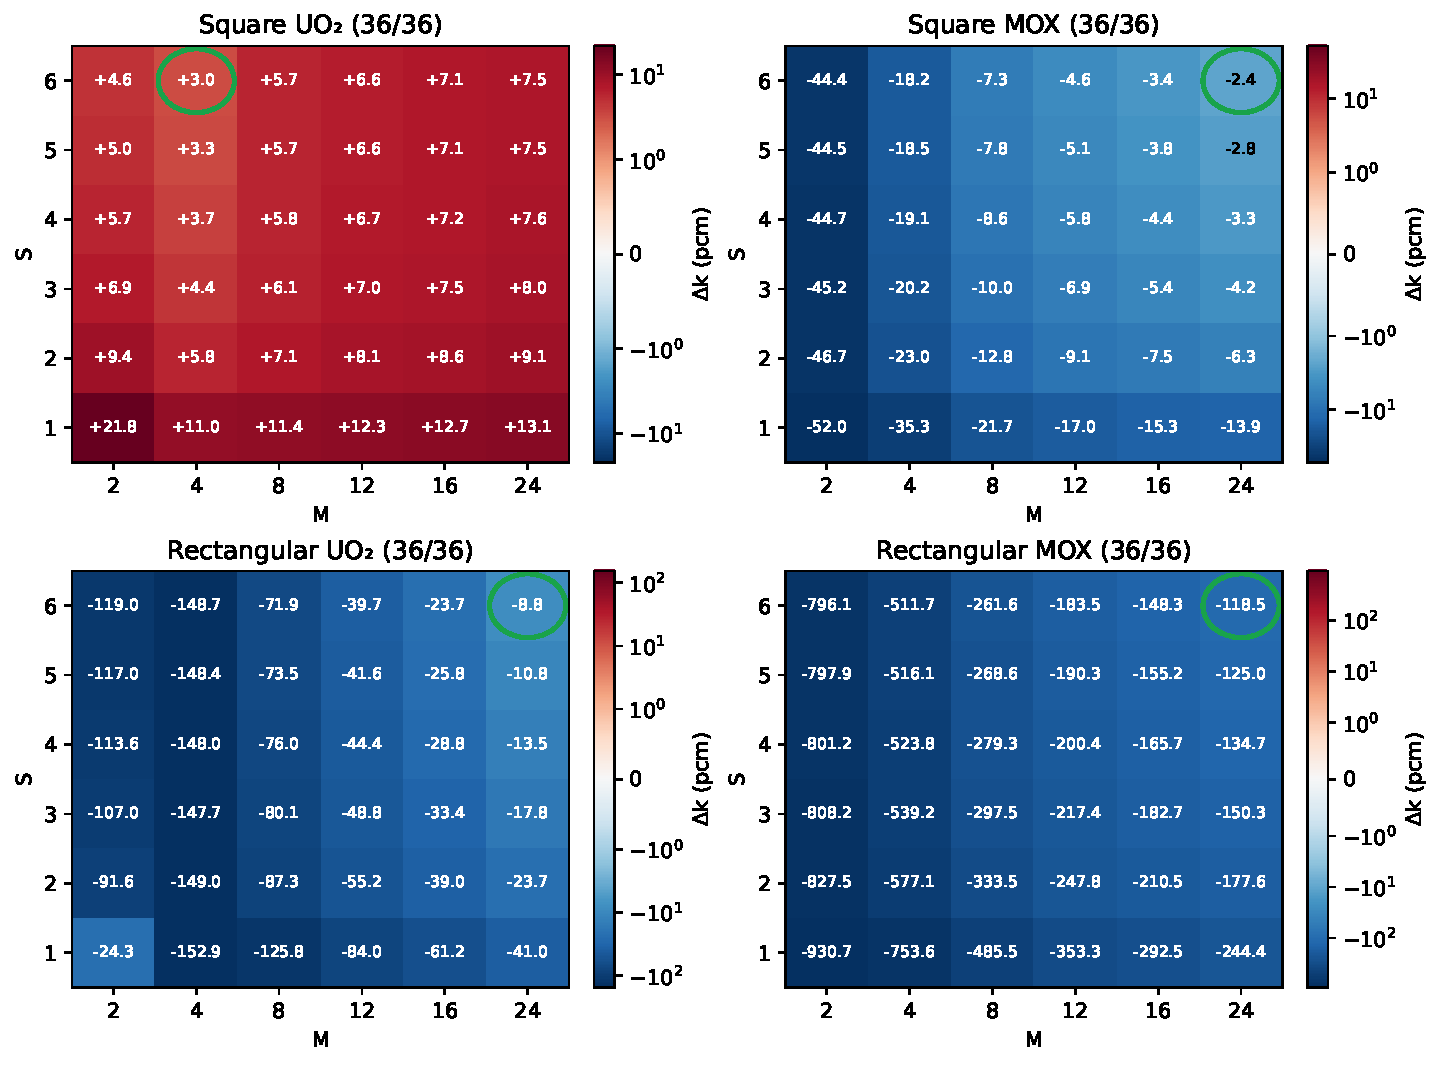
\includegraphics[width=.86\linewidth]{studyIII_c5g7_sm.pdf}
\caption{Signed eigenvalue differences for the pin-homogenised square and explicit
rectangular C5G7 assemblies, in pcm against each same-geometry OpenMC reference. The
marker indicates the smallest measured absolute difference in each panel.}
\label{fig:c5g7}
\end{figure}

\begin{figure}[htbp]
\centering
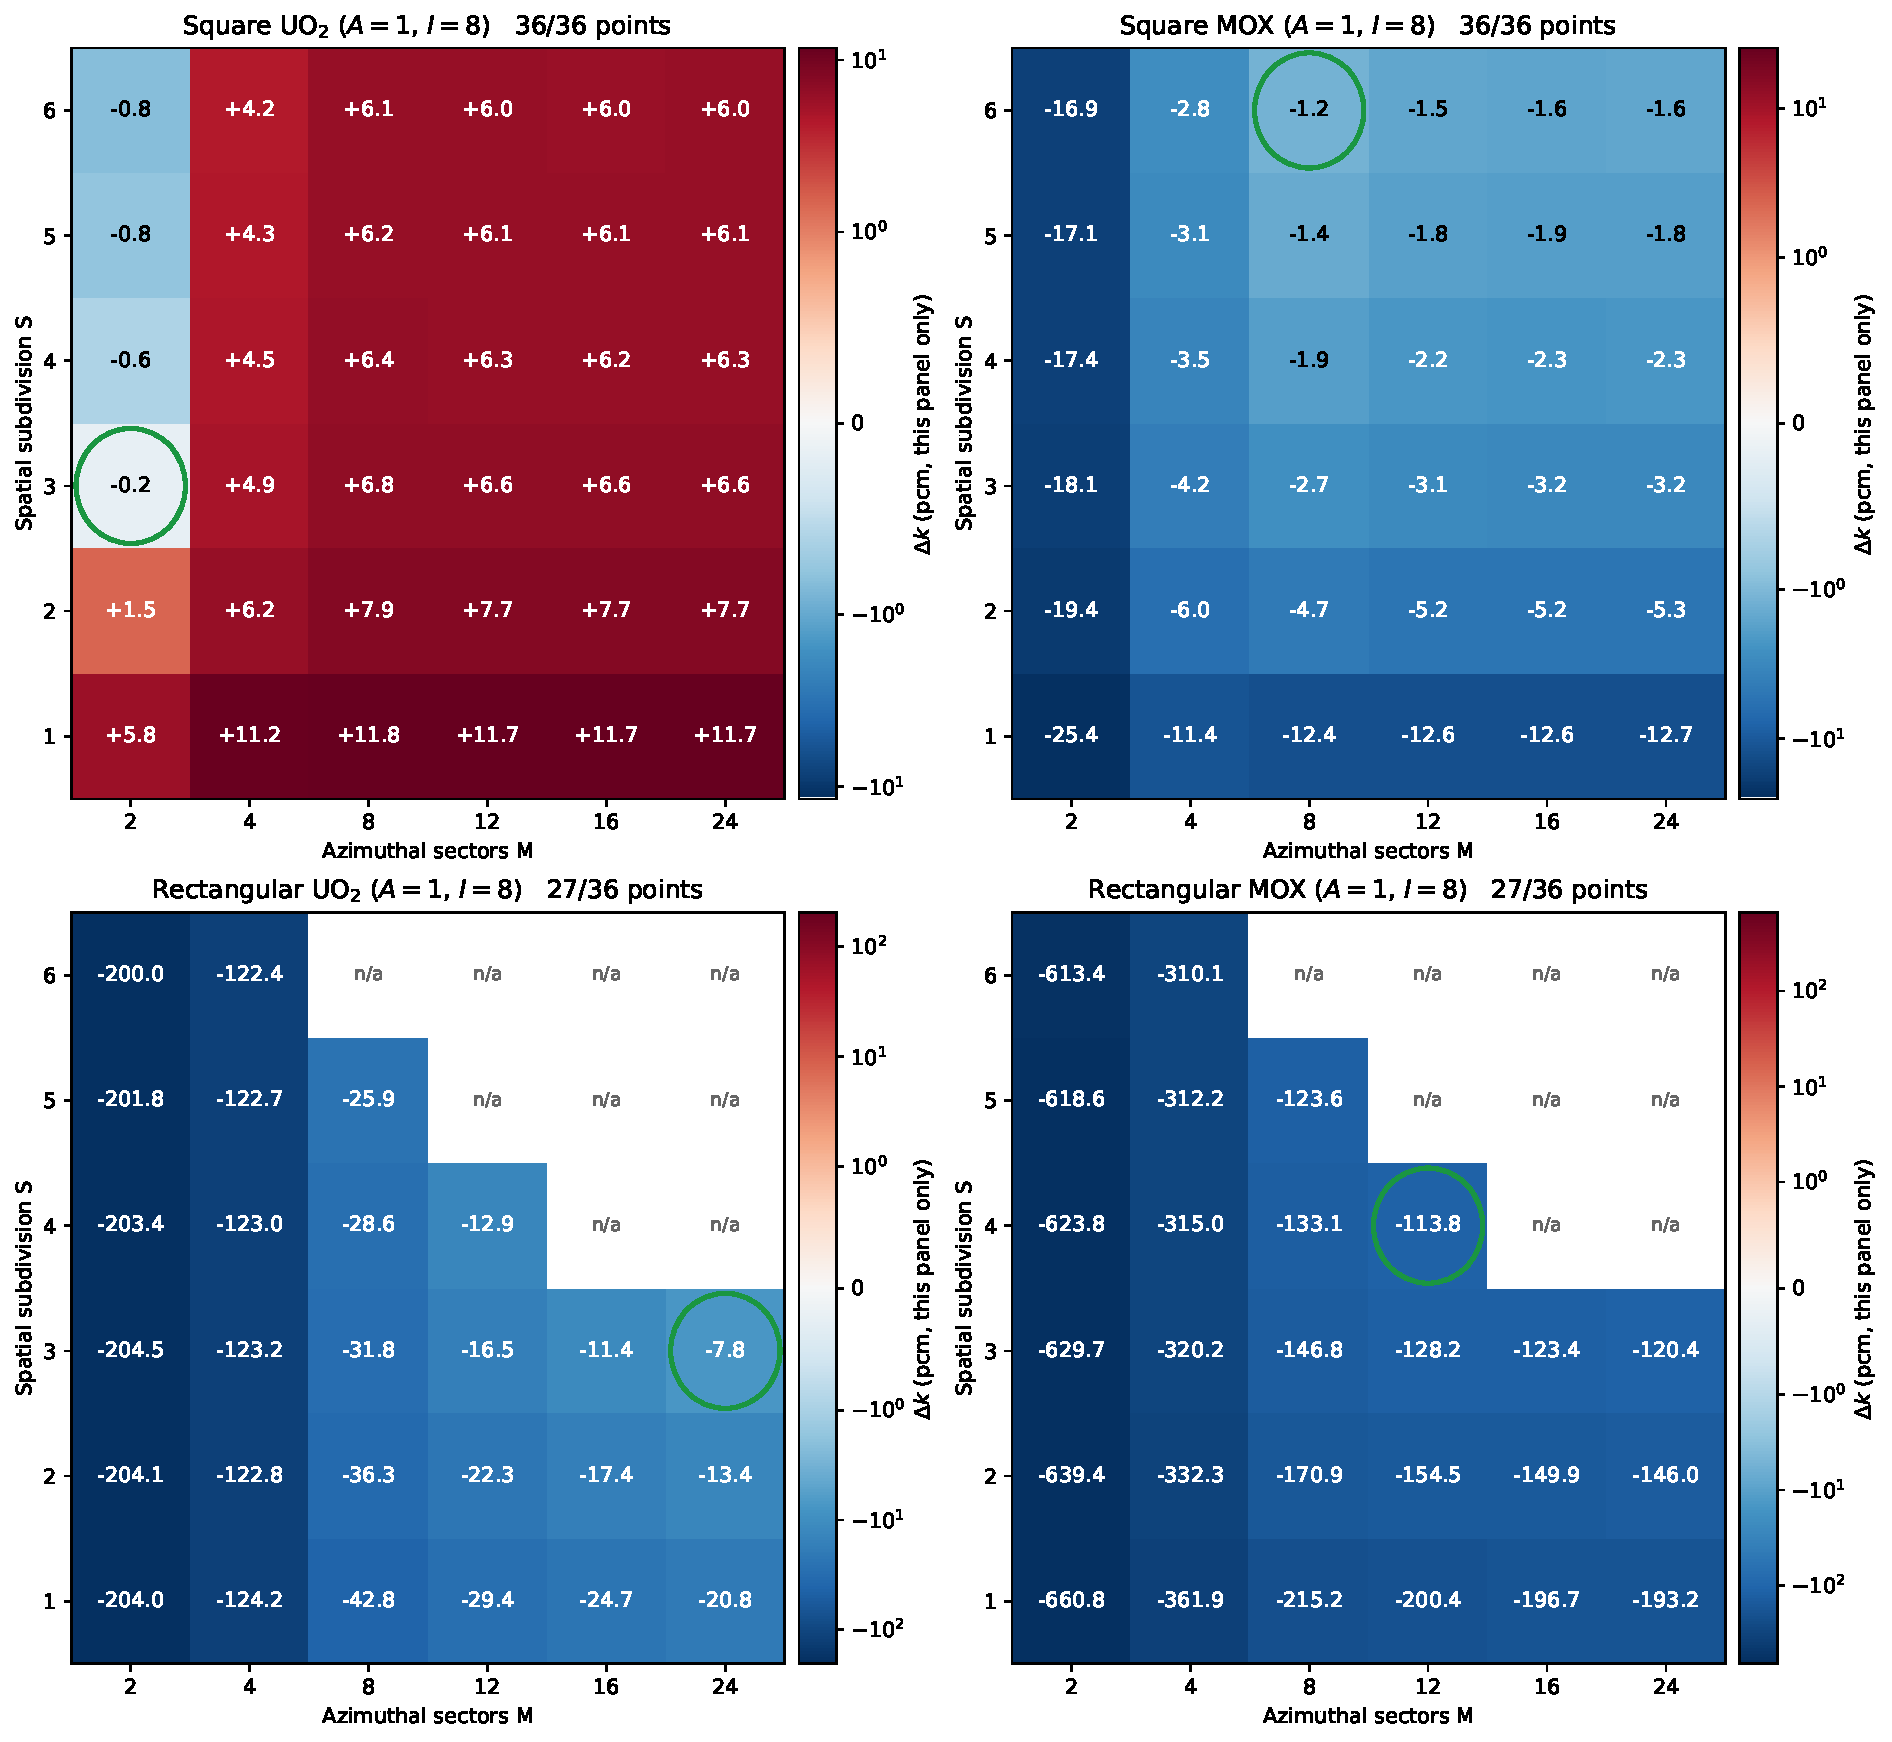
\includegraphics[width=\linewidth]{study4_assembly_grid2x2.pdf}
\caption{The same four matrices re-measured with the direction-wise closure: square
assemblies above, rectangular below, UO$_2$ left and MOX right, each panel drawn on its
own colour scale, so only the printed pcm values compare across panels. The ring marks
the smallest measured absolute difference of the panel.}
\label{fig:assembly-grid}
\end{figure}

\begin{figure}[htbp]
\centering
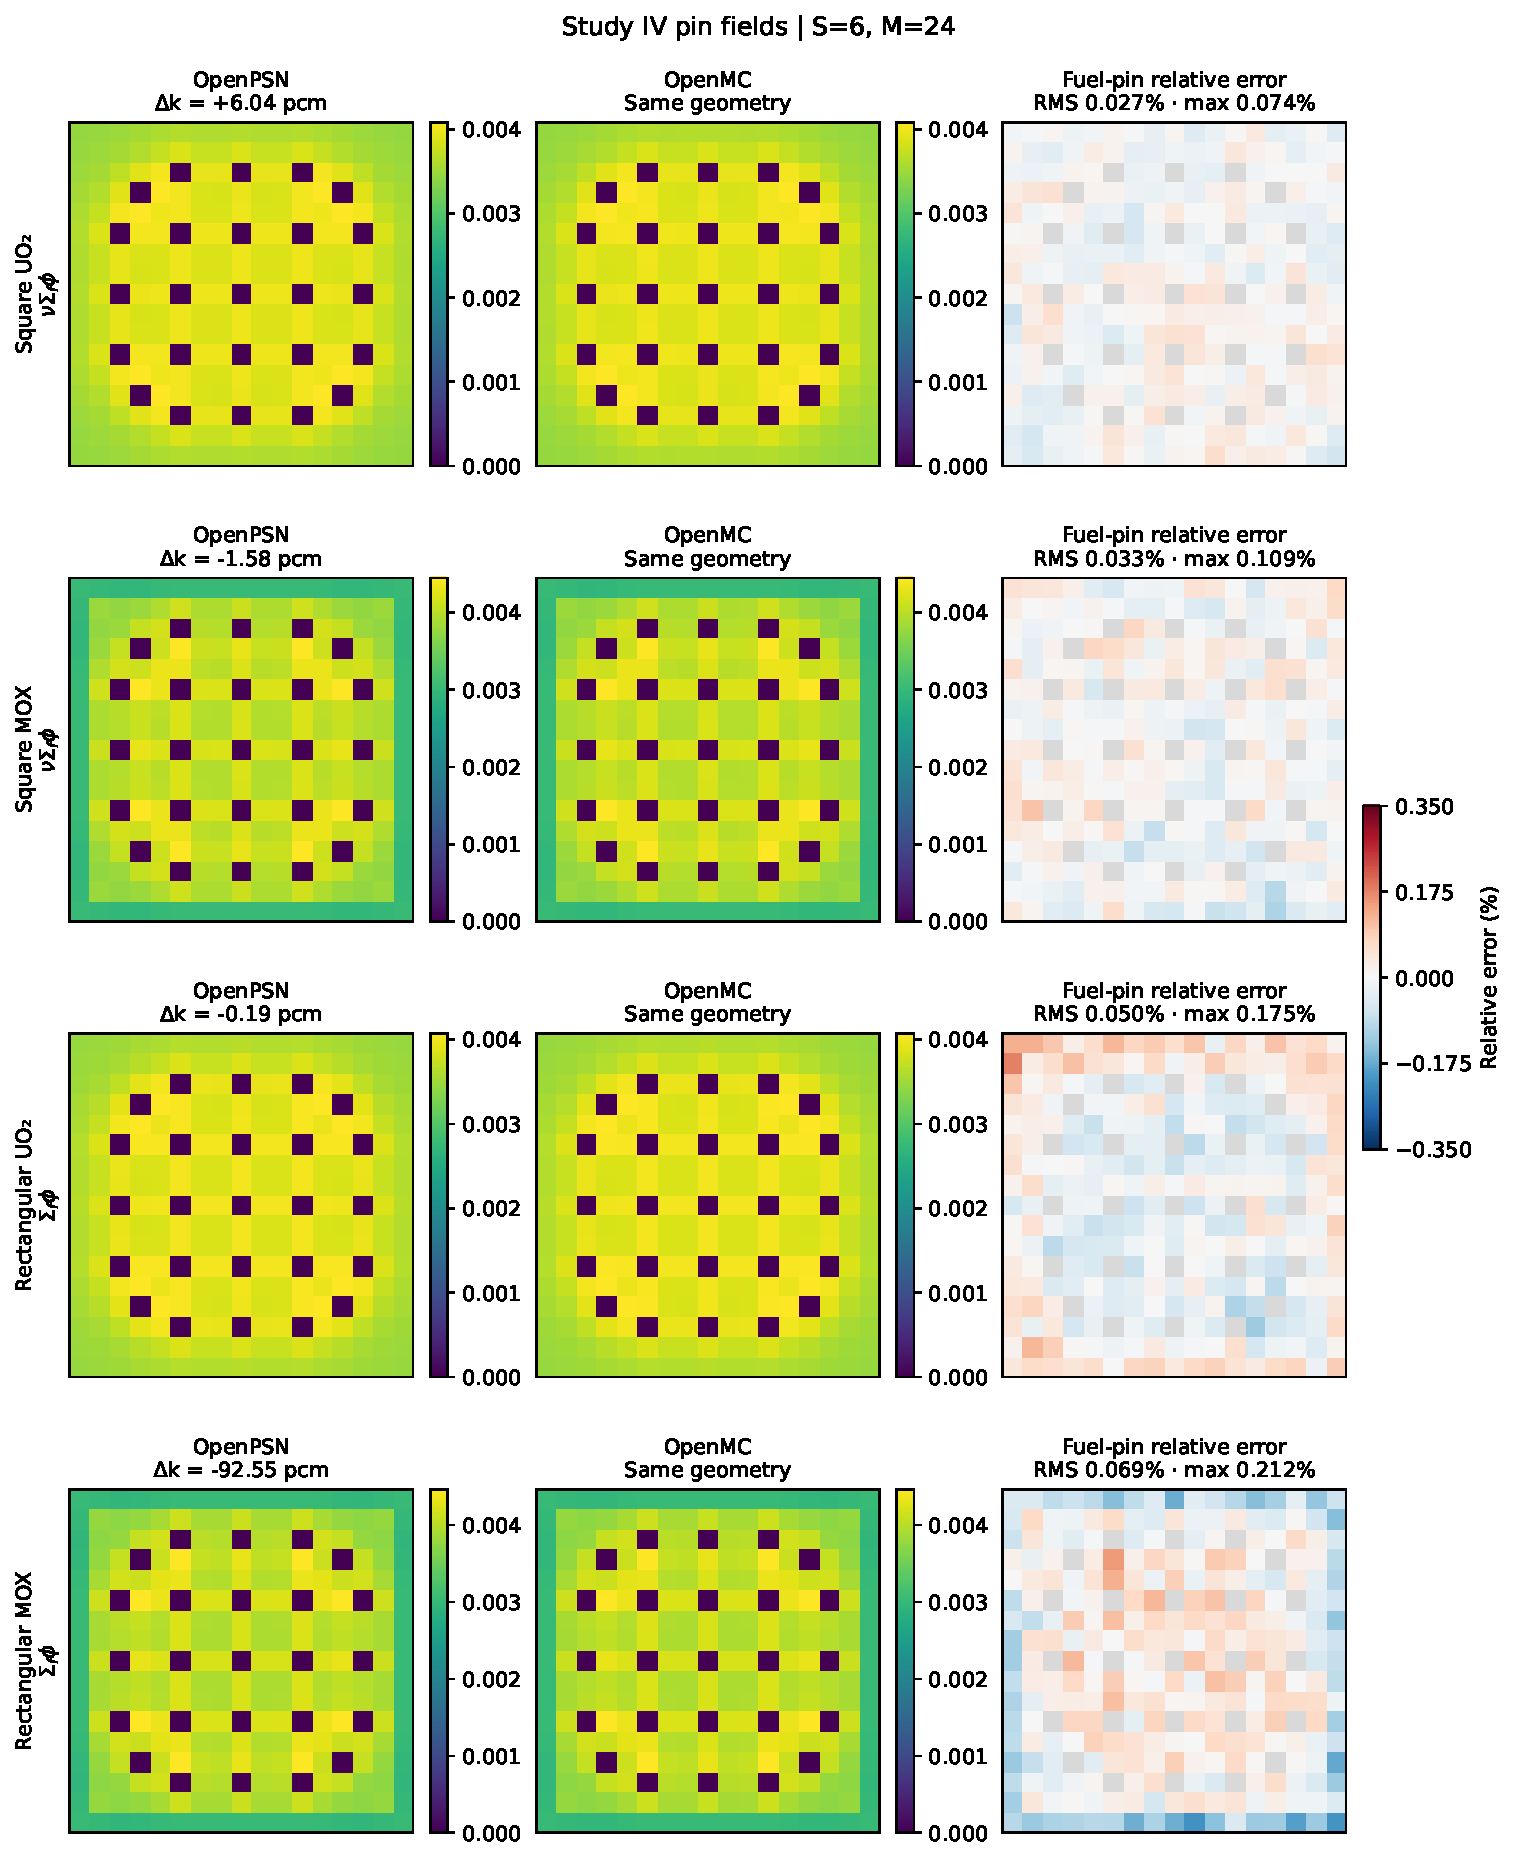
\includegraphics[width=.87\linewidth]{study4_assembly_fission.pdf}
\caption{Direction-wise assembly fields at the finest calculated grid, $S=6$, $M=24$,
with their OpenMC references and
relative errors over 264 fuel pins per case. Square maps show neutron production.
Rectangular maps use material-average neutron yields for the fission-rate conversion.
Each map is shifted by its minimum and normalised to unit pin sum. The relative-error
scale is $-0.35\%$ to $+0.35\%$ for all four assemblies and the quarter core.}
\label{fig:assembly-fields}
\end{figure}

The rectangular MOX bias remains of order $10^2\pcm$ at $A{=}1$ for both closures.
The trend suggests a
material-and-tiling effect rather than an angular one: at fixed $M{=}24$, $A{=}2$ and
one polar mode the difference falls from $-185.20\pcm$ at $S{=}1$ through $-115.02$
($S{=}2$) and $-68.35$ ($S{=}4$) to $-52.81\pcm$ at $S{=}6$, so spatial resolution of
the explicit water gaps, not additional azimuth, carries the improvement.

The rectangular UO$_2$ matrices contain one non-monotone step: with $A{=}1$ on the
uniform subinterval layout, moving from $M{=}2$ to $M{=}4$ makes the eigenvalue worse
by $57.33\pcm$ at $S{=}1$. Two changes that do not touch the angular rule reduce it.
Reassigning the six subintervals per pin axis from $2/2/2$ to $1/4/1$ --- the same
three material boundaries and the same total pin width, with the extra intervals
inside the widest subinterval, which is the fuel, via the benchmark flag
\texttt{-\/-balance-pin} --- brings the step down to $40.69\pcm$ and improves every
MOX and UO$_2$ row of that matrix; on the uniform layout, raising the azimuth degree
to $A{=}4$, again at $S{=}1$ and $I{=}8$, gives $-71.17\pcm$ at $M{=}2$ and
$-33.21\pcm$ at $M{=}4$, so the reversal disappears. The step is an interaction
between a coarse sector and coarse intra-cell spatial resolution, and it is reduced
by refining either side rather than by an angular-rule change. On the square UO$_2$
model, where the pin is homogenised and the cell carries no intra-cell material
interface, the same $M{=}2\to4$ move at $S{=}1$, $A{=}1$ is only $-10.84\pcm$ in the
bilinear subspace and $-0.06\pcm$ in the quadratic one --- an order of magnitude
smaller, and gone once the spatial basis can represent the cell.

With the direction-wise closure at $A{=}1$, the change from $M{=}2$ to $M{=}4$
raises $\keff$ in all six rows of both UO$_2$ geometries. At $S{=}2$ this brings
the rectangular difference from $-204.06$ to $-122.77\pcm$. The square difference
moves from $+1.46$ to $+6.25\pcm$. The absolute error shrinks in the rectangular
rows and grows in the square rows.

\begin{figure}[htbp]
\centering
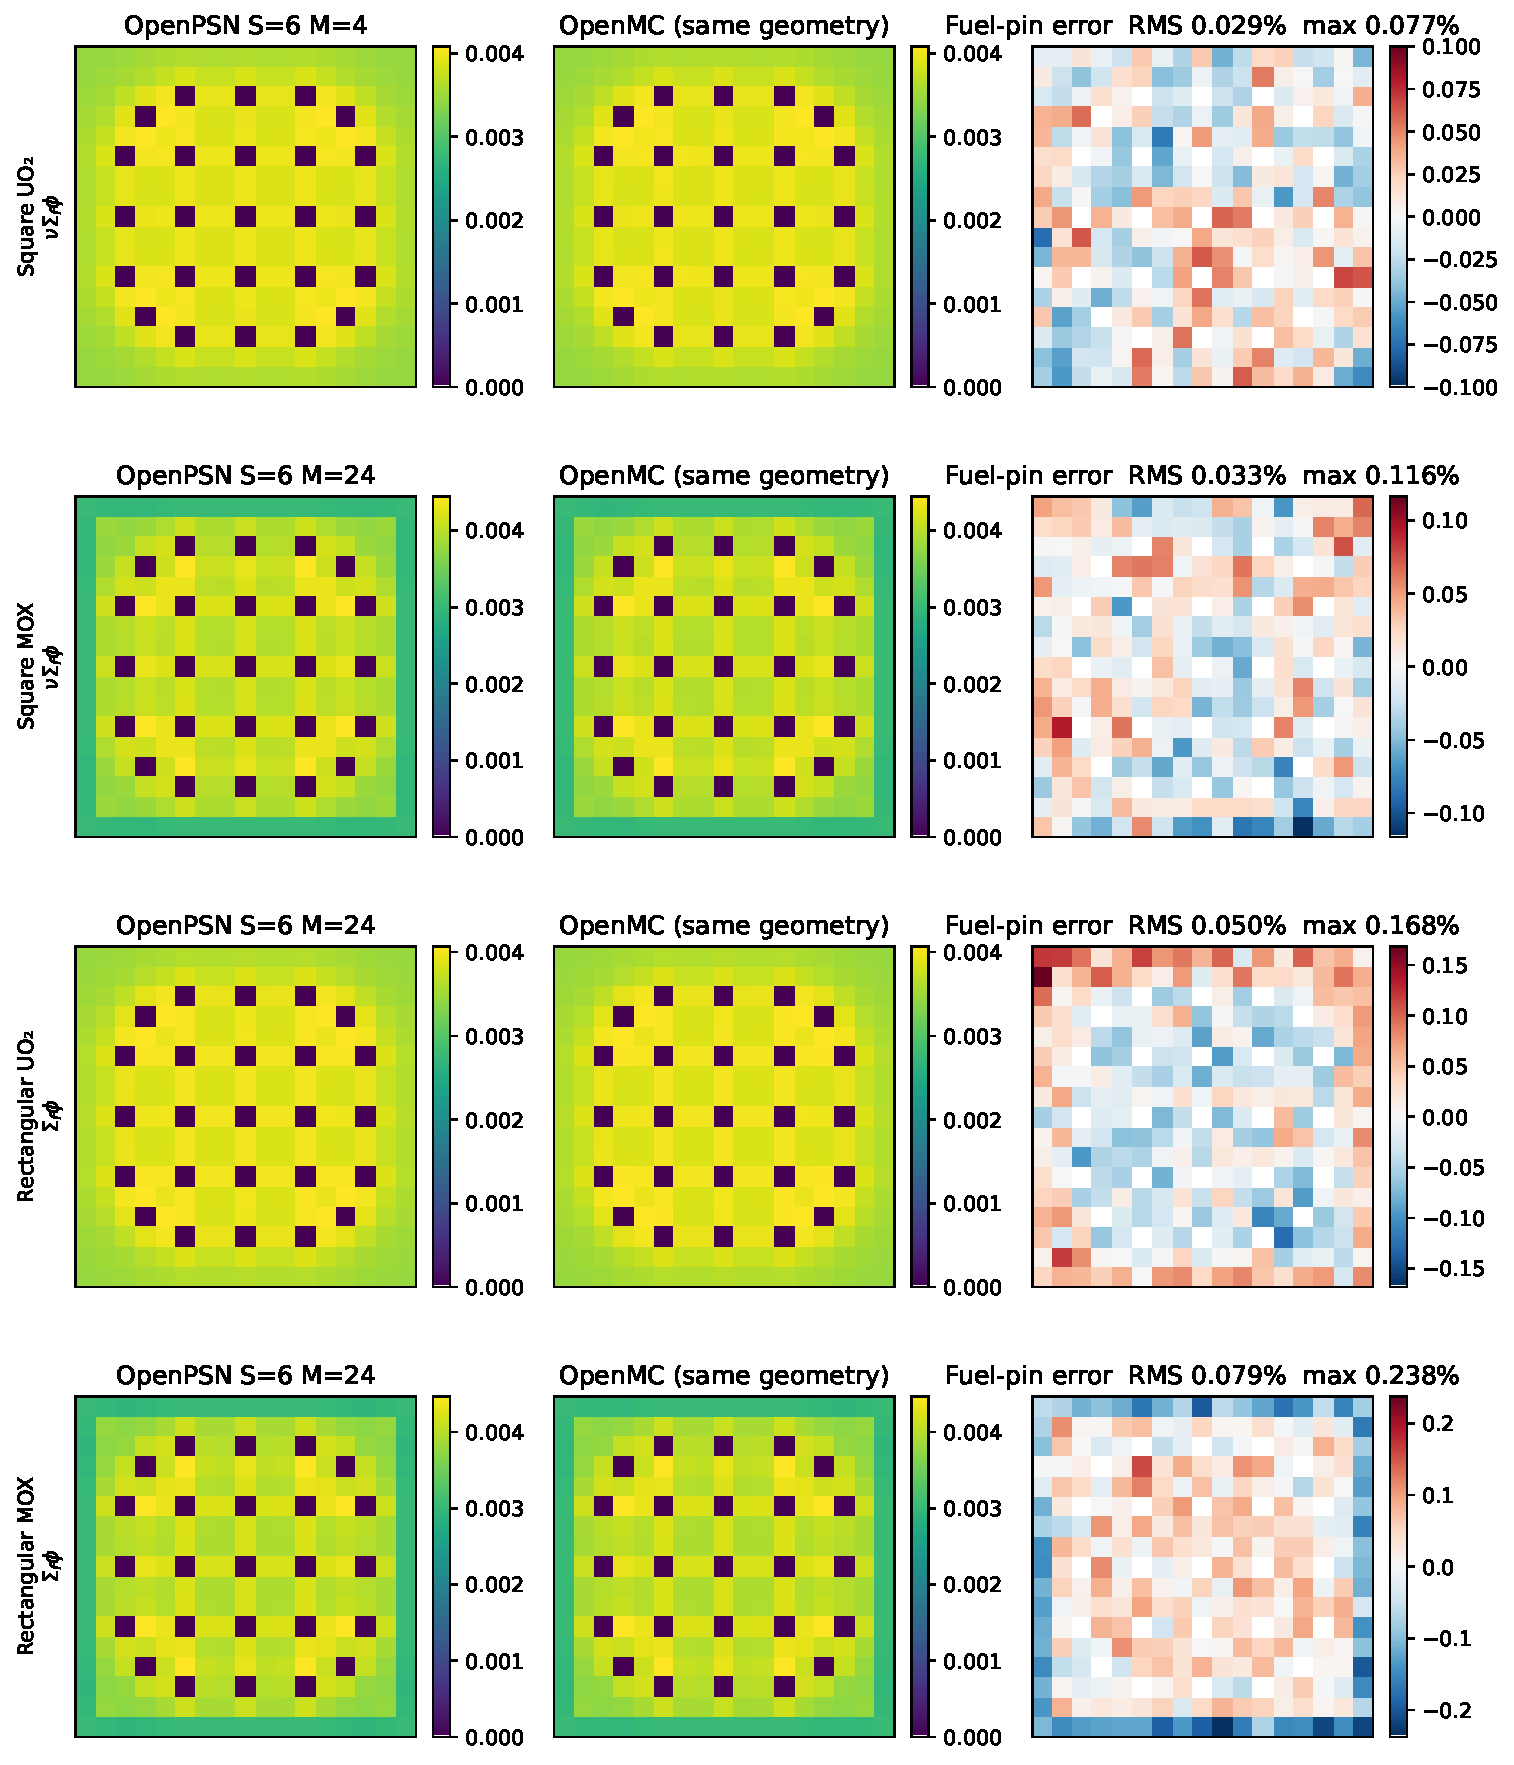
\includegraphics[width=.86\linewidth]{studyIII_best_fission.pdf}
\caption{Fuel-pin fission maps at the best measured assembly points, from left to
right OpenPSN, OpenMC and the relative pin error. The square rows use
$\nu\Sigma_f\phi$, the rectangular rows $\Sigma_f\phi$, each normalised to unit pin
sum.}
\label{fig:assembly-fission}
\end{figure}

\subsection{The explicit rectangular quarter core}
\label{sec:core}
The $5\times6$ grid of runs on the explicit quarter core, with the direction-wise
\texttt{sector\_diffusion} closure
(\texttt{c5g7\_rect\_quarter\_core.yaml}, seven groups, original material interfaces,
$(153S)^2$ nodes, TY3 polar rule, $A{=}1$, 60-thread cap) is given in
Tables~\ref{tab:study4-core-pcm} and \ref{tab:study4-core-time}. The reference is the
same-geometry OpenMC batch mean $1.187217554586068$ with a $3.41\pcm$ standard error
over 20{,}000 active batches; the statepoint \texttt{k\_combined} estimator is
$1.187220349151050$ with $1.75\pcm$. Each measured cell was solved independently and
re-verified by a separate transport sweep, and every cell of the $5\times6$ grid
converged.

\begin{table}[htbp]
\centering
\caption{Signed eigenvalue difference $10^{5}(\keff-k_\mathrm{ref})$ in pcm on the explicit quarter core, against the same-geometry OpenMC reference $1.187217554586$ ($3.41\,\mathrm{pcm}$ standard error). Bold marks the smallest measured absolute difference.}
\label{tab:study4-core-pcm}
\begin{tabular}{rrrrrrr}
\hline
 & \multicolumn{6}{c}{Azimuth sectors $M$}\\
\cline{2-7}
$S$ & 2 & 4 & 8 & 12 & 16 & 24\\
\hline
1 & -271.73 & -149.28 & -68.90 & -60.26 & -57.21 & -54.09 \\
2 & -263.55 & -137.20 & -49.66 & -40.31 & -37.10 & -33.95 \\
3 & -260.06 & -133.29 & -39.46 & -28.91 & -25.68 & -23.05 \\
4 & -257.30 & -131.26 & -33.57 & -22.58 & -19.44 & -16.77 \\
5 & -254.69 & -130.03 & -29.34 & -18.52 & -15.85 & \textbf{-12.98} \\
\hline
\end{tabular}
\end{table}

\begin{table}[htbp]
\centering
\caption{End-to-end wall time in seconds for the same points, including assembly, factor construction, outer iterations and the verification sweep. An asterisk marks a point that reused a stored factorisation. Points sharing a time window ran concurrently, so the column reports load rather than throughput.}
\label{tab:study4-core-time}
\begin{tabular}{rrrrrrr}
\hline
 & \multicolumn{6}{c}{Azimuth sectors $M$}\\
\cline{2-7}
$S$ & 2 & 4 & 8 & 12 & 16 & 24\\
\hline
1 & 77.8 & 113.4 & 166.4 & 176.1 & 237.8 & 340.7 \\
2 & 625.3 & 790.3 & 548.5 & 1299.0 & 996.6 & 1810.2 \\
3 & 1199.5 & 1757.3 & 1559.8 & 1787.4 & 2790.4 & 2518.8 \\
4 & 3263.4 & 1647.5 & 3486.0 & 2665.9 & 2163.1* & 4360.9 \\
5 & 5787.4 & 3161.0 & 3440.0 & 5084.0 & 4841.3* & 10930.6* \\
\hline
\end{tabular}
\end{table}


\begin{figure}[htbp]
\centering
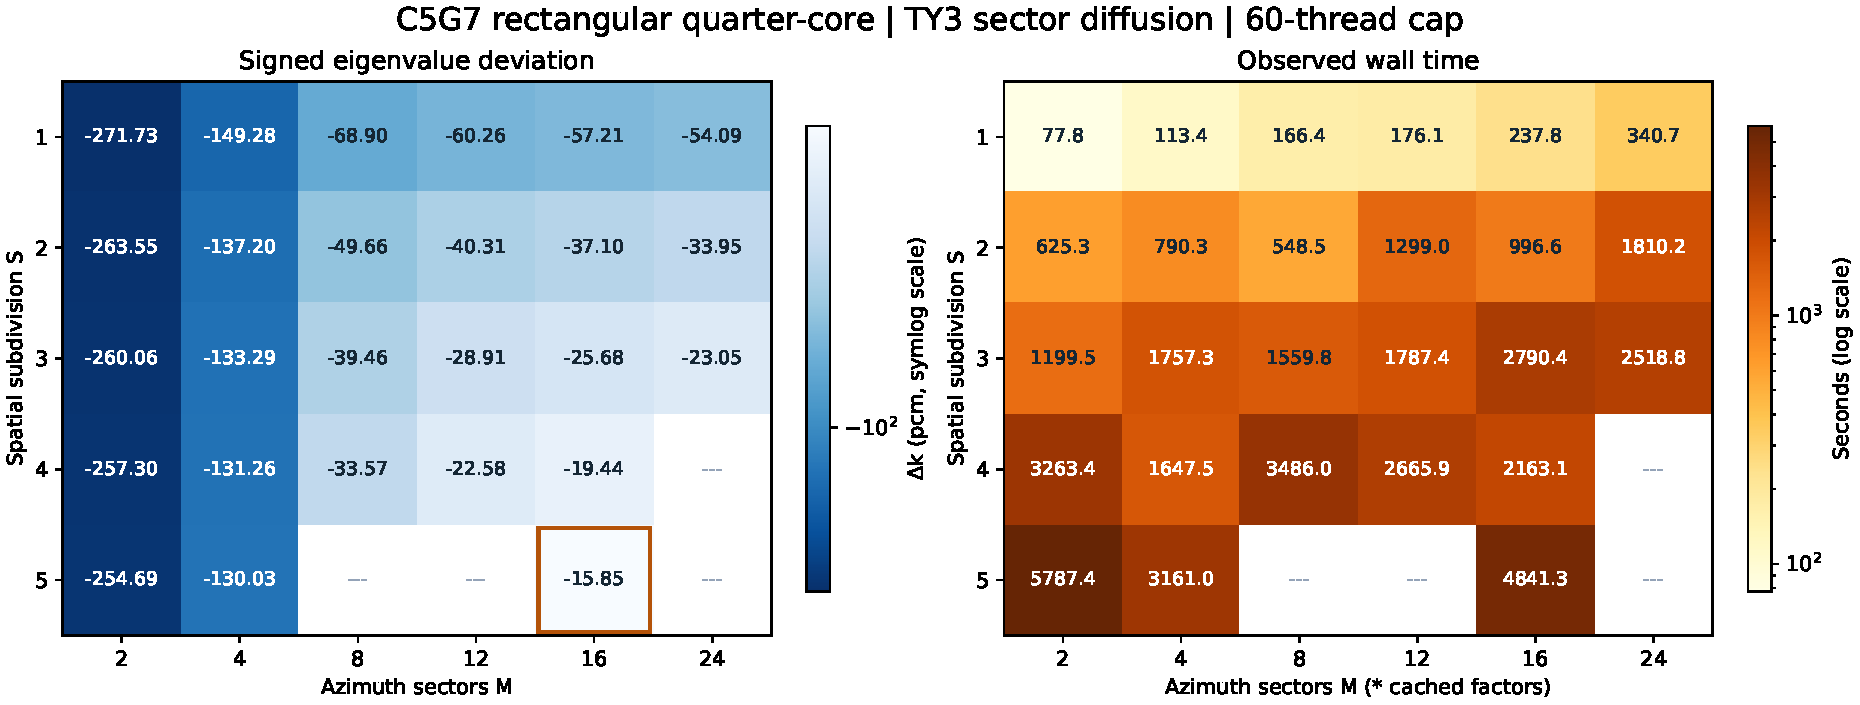
\includegraphics[width=\linewidth]{sector_diffusion_sm.pdf}
\caption{The measured quarter-core matrices. Left: signed eigenvalue difference in pcm
(symlog scale), the framed cell marking the smallest absolute difference. Right:
end-to-end wall time in seconds (log scale).}
\label{fig:core}
\end{figure}

The error is one-signed over the whole measured grid and decreases as either axis is
refined --- all 49 adjacent refinement steps of the completed grid move it toward zero ---
and the smallest measured difference is $-12.98\pcm$ at $S{=}5$, $M{=}24$, with a
relative pin-wise fission-rate difference over the 1056 fuel pins of RMS $0.084\%$ and
maximum $0.321\%$ (Table~\ref{tab:study4-core-best}, Figure~\ref{fig:core-fission}).
Two effects of comparable size must be read with these numbers. OpenPSN reads the
C5G7 fission spectrum as supplied, with $\sum_g\chi_g=1.00000917761$, whereas OpenMC
renormalises it on read; since $k_\text{raw}=(\sum_g\chi_g)k_\text{normalised}$, this
input convention alone shifts the present reference by $1.0896\pcm$. And the reference
itself carries $3.39$--$3.91\pcm$ of statistical uncertainty for block sizes of 10 to
500 batches. Both are smaller than the residual bias, which is why the comparison is
reported cell by cell rather than as a single number.

\begin{table}[htbp]
\centering
\caption{The cell of Table~\ref{tab:study4-core-pcm} with the smallest absolute
eigenvalue difference, with a relative pin-wise fission-rate difference of RMS 0.084\% and maximum absolute value 0.321\%. The node count is $(153S)^2$.}
\label{tab:study4-core-best}
\begin{tabular}{lr}
\hline
spatial subdivision $S$ & 5\\
azimuth sectors $M$ & 24\\
nodes & 585225\\
$\keff$ & 1.187087778706\\
$\Delta k$ & $-12.98\pcm$\\
wall time & 10930.6~s (stored factors)\\
\hline
\end{tabular}
\end{table}


\begin{figure}[htbp]
\centering
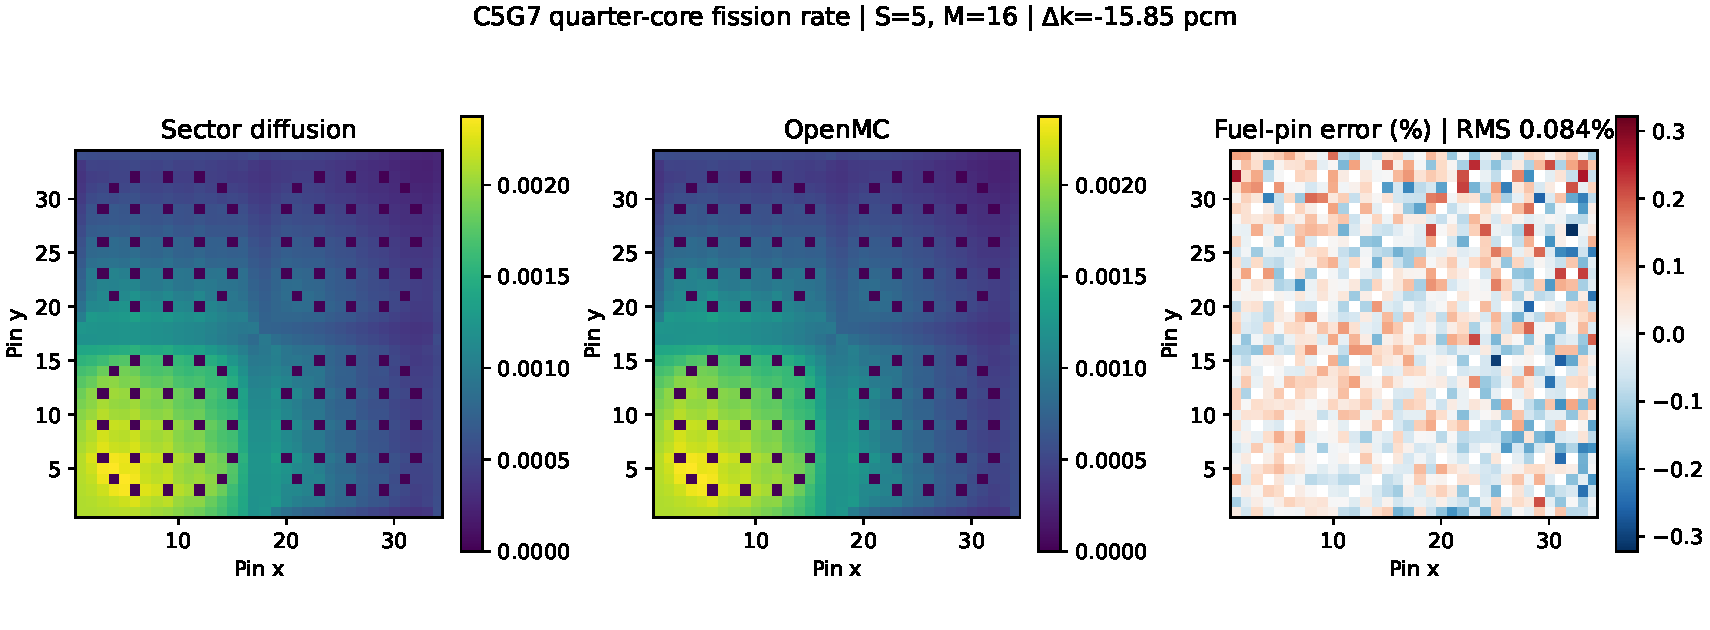
\includegraphics[width=\linewidth]{study4_core_fission.pdf}
\caption{Normalised fuel fission rate at the finest calculated quarter-core grid,
$S=5$, $M=24$, beside the same-geometry OpenMC reference and the relative difference over
the 1056 fuel pins. The error scale is $-0.35\%$ to $+0.35\%$.}
\label{fig:core-fission}
\end{figure}

How far the remaining bias is azimuthal was estimated on the same base grid at $I{=}8$
polar nodes and $A{=}1$: the successive increments $M{=}4,8,16$ and $M{=}8,16,32$ give
local azimuthal orders of $1.32$ and $1.47$, and the two windows extrapolate to
$-54.64\pcm$ and $-58.90\pcm$ as $M\rightarrow\infty$ at fixed spatial and polar
resolution. In a separate test at $M{=}16$, refining the $172\times172$ graded mesh
to $244\times244$ moves $\keff$ by $3.24\pcm$. Those tests leave a substantial residual
at fixed polar order. The TY3 uniform refinement in Table~\ref{tab:study4-core-pcm}
continues to improve through its finest measured point, $S{=}5$, $M{=}24$.

\subsection{Cost at equal angular resolution}
\label{sec:cost}
On the $153\times153$ rectangular assembly grid at $I{=}8$, $S{=}1$, a 60-thread cap
and a 45~GiB factor-pool limit, with the legacy path on \texttt{chol-packed-rs} and
the sector closure on \texttt{sector-cholmod}, the recorded end-to-end times are:

\begin{table}[htbp]
\centering
\caption{End-to-end seconds and eigenvalue difference on the rectangular assembly at
$S{=}1$, $I{=}8$, one point after another on one host. The sector columns use $A{=}1$.}
\label{tab:cost}
\centering\small
\begin{tabular}{r l l l}
\hline
$M$ & legacy & bilinear coefficients & quadratic coefficients \\
\hline
8  & $60.21$~s / $-203.73\pcm$ & $50.26$~s / $-200.95\pcm$ & $59.12$~s / $-123.55\pcm$ \\
16 & $82.32$~s / $-78.52\pcm$  & $73.12$~s / $-114.13\pcm$ & $160.49$~s / $-82.27\pcm$ \\
\hline
\end{tabular}
\end{table}

\begin{table}[htbp]
\centering
\caption{Cost of the two closures at equal angular unknowns.  Each pair was run
through \texttt{scripts/sector\_diffusion\_benchmark.py} on one host, one closure
immediately after the other, at the same $M$, $A$, $I$, thread budget, factor kernel
and memory cap (8 threads, 10~GiB,
\texttt{sector-cholmod}); the load average at the start of each run is in the data
file, and the host was also carrying the rest of the campaign, so these are workload
records.  $s$ is the end-to-end time, pcm the difference from the same reference.
Median ratio 0.98 over 10 pairs.}
\label{tab:study4-closure-cost}
\centering\small
\begin{tabular}{l r r l l r}
\hline
Case & $(S,M)$ & $A$ & \texttt{sector\_average} & \texttt{sector\_diffusion} & ratio \\
\hline
Square MOX & $(4,8)$ & $1$ & 23.32~s / -6.09 & 22.90~s / -1.85 & 0.98\\
Square UO$_2$ & $(4,8)$ & $1$ & 20.29~s / +6.24 & 15.70~s / +6.39 & 0.77\\
Strong absorber & $(4,8)$ & $2$ & 0.69~s / -100.79 & 0.48~s / -76.46 & 0.70\\
Strong absorber & $(8,16)$ & $1$ & 2.29~s / -48.45 & 2.17~s / -23.02 & 0.95\\
Strong absorber & $(12,24)$ & $0$ & 3.84~s / -107.43 & 3.29~s / -9.97 & 0.86\\
Strong absorber & $(12,24)$ & $1$ & 5.10~s / -34.13 & 7.38~s / -12.25 & 1.45\\
Weak absorber & $(4,8)$ & $2$ & 0.69~s / -19.78 & 0.36~s / -15.21 & 0.52\\
Weak absorber & $(8,16)$ & $1$ & 2.35~s / -10.40 & 2.40~s / -5.65 & 1.02\\
Weak absorber & $(12,24)$ & $0$ & 3.06~s / -21.61 & 3.43~s / -3.35 & 1.12\\
Weak absorber & $(12,24)$ & $1$ & 5.05~s / -7.85 & 6.22~s / -3.73 & 1.23\\
\hline
\end{tabular}
\end{table}


Against the \emph{legacy} path, the measured sector-to-legacy time ratio is $2.7$ on
the quarter core and $0.83$--$1.95$ on the assembly grid of Table~\ref{tab:cost}, where
the paths use different factor kernels. The \emph{two sector closures} use the same
number of angular unknowns at equal $A$ and $M$. Over the ten pairs of
Table~\ref{tab:study4-closure-cost}, run sequentially on one host, the median
direction-wise to cell-average time ratio is $0.98$, with a range of $0.52$--$1.45$.

Table~\ref{tab:cost} says the sector closure is affordable but not free, and it does
not order the two paths by accuracy: at $M{=}16$ the cheaper bilinear representation
is the less accurate of the two sector runs. The same pattern appears on the quarter
core, where at identical geometry, grid, thread budget and a cold start the legacy
closure at $S{=}1$, $M{=}24$ gives $-10.12\pcm$ in $128.08$~s and the sector closure
$-54.09\pcm$ in $340.68$~s. At the coarsest settings the legacy node model has the
smaller error at equal angular resolution; the tables of Sections
\ref{sec:checker}--\ref{sec:core} show the sector error decreasing as either axis is
refined, which is the regime where the two paths cross. A matched-cost comparison, in
which cost is fixed and both paths are refined to that cost, was not performed.

\section{Discussion and scope}
\label{sec:scope}

What the measurements establish is narrow and checkable: with the face closure taken
from the same weak form as the body term, the sign-changing valley of the square
checkerboard does not appear anywhere in the 314 points of the direction-wise closure of
record except its one $A{=}1$, $M{=}4$ column, the error outside that column is
one-signed and moves toward zero at 246 of the 280 refinements of the spatial axis ---
the 34 that do not all lie in that column --- keeping the
direction-wise error below the cell-average one at \StudyFourSmaller{} of the \StudyFourPairs{} paired points at equal
angular unknowns. The nodal-response rewriting is an exact algebraic identity
on the same discrete system.
On the quarter core the absolute eigenvalue difference decreases along both axes at
all 49 adjacent refinements. Its best pin-wise fission field differs from the reference
by $0.084\%$ RMS.

What they do not establish should be read off the same tables. The quarter-core matrix
is a measured grid, not a convergence proof: its best cell still differs from the
Monte Carlo reference by more than that reference's own standard error, and the
azimuthal extrapolation of Section~\ref{sec:core} suggests that angular refinement
alone will not close the remaining bias. The rectangular MOX assembly keeps a bias of
order $100\pcm$ at the best $A{=}1$ setting. The direction-wise
matrices of the two rectangular cases are also the least complete part of the archive:
each is short of nine cells, one of which --- $(S,M){=}(6,24)$ --- is the archived
closure's own best point of that case, so their measured bests are lower bounds on what
the closure can do there rather than its limits. The sector closure costs $2.7$ times the
legacy path on the quarter core at $S{=}1$, $M{=}24$ ($340.68$~s against $128.08$~s,
both cold), while on the assembly grid its bilinear representation runs faster than
the legacy path at the same $M$ and its quadratic representation slower; the two paths
also use different factor kernels there, so those entries are workload records rather
than throughput measurements, because points shared a host and some reused stored
factors.
The exact checks constrain the operator and the algebra of the assembly, not the
truncation error of a production mesh. Items known to be missing from the archive ---
the Monte Carlo statepoint and batch statistics behind the quarter-core reference, and
two numbers removed from an earlier draft for lack of a reproducible source --- are
listed in \texttt{paper/unresolved\_items.md}.

\section{Conclusions}

A finite-sector closure of the even-parity equation, in which the diffusion tensor of
each finite angular cell is the exact second moment of the retained directions and the
interface and vacuum terms come from the same weak form as the body term, removes the
sign-changing diagonal valley of the published PSN checkerboard error survey at 279 of
the 314 points tested with it --- every point but one under-resolved azimuthal column
--- with an error that is one-signed outside that column and moves toward zero at 246 of
the 280 refinements of the spatial axis, all 34 exceptions again inside that column.
Measured point by point against the cell-average
reduction of the same tensor at the same $A$, $S$, $M$ and $I$, it is the more accurate
of the two at \StudyFourSmaller{} of \StudyFourPairs{} points, at a median error ratio of $\StudyFourMedianRatio$ and a median time
ratio of $0.98$. The same closure, run as $S\times M$ grids on the four C5G7 assemblies
and the explicit rectangular quarter core, gives eigenvalue differences from
same-geometry Monte Carlo references, reaching $-0.16$ and
$-1.20\pcm$ on the pin-homogenised square assemblies ($+3.02$ and $-2.45\pcm$ for the
archived closure there) and $-12.98\pcm$ on the
quarter core, where the pin-wise fission field differs by $0.084\%$ RMS. The residual
differences are attributed, with supporting sweeps, to intra-cell material and polar
resolution and to the coarse-sector interaction that produces the $M{=}2\rightarrow4$
step, not to the number of azimuth sectors. The construction keeps its unknowns on
finite cells of the sphere, and its exactness claims are confined to the algebra up to
the chosen discrete spaces, which is what the two counterexamples of
Section~\ref{sec:method} make necessary.

\section*{Reproducibility}
All runs are produced by \texttt{scripts/sector\_diffusion\_benchmark.py}; the archived
per-point logs are in \texttt{examples/psn\_repro/logs/} and
\texttt{examples/c5g7/study4\_sector\_core/logs/}, the per-point result files in
\texttt{paper/data/}, and the exact checks in \texttt{examples/psn\_strict\_checks/}.
Every table in this paper is written by
\texttt{scripts/\allowbreak study4\_\allowbreak checkerboard\_\allowbreak report.py},
\texttt{scripts/\allowbreak study4\_\allowbreak assembly\_\allowbreak report.py} or
\texttt{scripts/\allowbreak study4\_\allowbreak core\_\allowbreak report.py}
from those files, with assertions on closure, angular degrees, quadrature, node count,
reference value, residuals and the internal consistency of each reported pcm value; a
missing or inconsistent run stops the build. The exact checks and the regressions run
with
\begin{quote}\small\ttfamily
cd examples/psn\_strict\_checks\\
python -m unittest discover -s . -p 'test\_*.py'\\
python -m unittest tests/test\_sector\_diffusion.py\\
python tests/run\_examples.py
\end{quote}
and the optional SuiteSparse backend, whose only effect is speed, is built with
\begin{quote}\small\ttfamily
cc -O3 -fPIC -shared -I/usr/include/suitesparse \\
\ \ \ \ psn2d/sector\_cholmod.c -lcholmod \\
\ \ \ \ -o psn2d/libsector\_cholmod.so
\end{quote}
The branch \texttt{psn-4} of
\texttt{github.com/xycjscs/OpenPSN} contains the code, inputs, logs, result files and
generation scripts.

\begin{thebibliography}{9}
\small

\bibitem{openpsn2026}
Y.~Xu, ``OpenPSN: Implementation, Verification, and Assessment of Nodal Transport
Methods,'' preprint (September 2026), \texttt{github.com/xycjscs/OpenPSN}.

\bibitem{psn2027}
Y.-A.~Chao, Z.~Li, and G.~Chen, ``Diffusion-based phase space nodal method (PSN):
Solving the neutron transport equation with a diffusion code,'' \emph{Annals of
Nuclear Energy} \textbf{240} (2027) 112707 \doi{10.1016/j.anucene.2026.112707}.

\bibitem{ghazaie2019mpn}
S.~H.~Ghazaie, M.~Abbasi, and A.~Zolfaghari, ``The Multi-PN approximation to neutron
transport equation,'' \emph{Progress in Nuclear Energy} \textbf{110} (2019) 64--74
\doi{10.1016/j.pnucene.2018.09.001}.

\bibitem{falabino2022mpn}
M.~Falabino, D.~Sciannandrone, E.~Masiello, and J.-F.~Vidal, ``The Multi-PN angular
discretization method of the neutral-particle transport equation for radiation
shielding calculations,'' \emph{Annals of Nuclear Energy} \textbf{177} (2022) 109301
\doi{10.1016/j.anucene.2022.109301}.

\bibitem{nea2003}
\emph{Benchmark on Deterministic Transport Calculations Without Spatial
Homogenisation: A 2-D/3-D MOX Fuel Assembly Benchmark}, OECD/NEA NSC document
NEA/NSC/DOC(2003)16 (2003).

\bibitem{c5g7td}
J.~Hou, K.~N.~Ivanov, V.~F.~Boyarinov, and P.~A.~Fomichenko, ``OECD/NEA benchmark for
time-dependent neutron transport calculations without spatial homogenization,''
\emph{Nuclear Engineering and Design} \textbf{317} (2017) 177--189
\doi{10.1016/j.nucengdes.2017.02.008}.

\bibitem{openmc2015}
P.~K.~Romano, N.~E.~Horelik, B.~R.~Herman, A.~G.~Nelson, B.~Forget, and K.~Smith,
``OpenMC: A state-of-the-art Monte Carlo code for research and development,''
\emph{Annals of Nuclear Energy} \textbf{82} (2015) 90--97
\doi{10.1016/j.anucene.2014.07.048}.

\end{thebibliography}

\appendix
\section*{Appendix A. Notation, angular sets and check inventory}
\addcontentsline{toc}{section}{Appendix A}

\textbf{Notation.} $S$ is the number of spatial subdivisions per material interval
(the quarter core uses $(153S)^2$ cells), $M$ the number of azimuth sectors per
half-plane, $A$ the degree of the local azimuthal basis inside a sector (so each
sector carries $A{+}1$ Gauss directions), $I$ the number of polar nodes ($I/2$ per
half-axis for Gauss polar nodes; TY3 uses a fixed three-point rule per band), and
$\Delta k=10^{5}(\keff-k_\mathrm{ref})$ in pcm.

\textbf{Angular sets actually used.} Checkerboard scans $I{=}30$ with Gauss polar
nodes; assembly scans $I{=}8$; quarter core TY3 with $A{=}1$; the azimuthal-order and
quadrature-failure studies use $I{=}8$ with $A{=}1$ and, for the failure trial, two
quadrature points per sector. The slope space is biquadratic unless a row states
``bilinear''; the mixed \texttt{quadratic-linear} option was used only in exploratory
runs and no number in this paper depends on it.

\textbf{Exact checks} (\texttt{examples/psn\_strict\_checks}, 14 items): two-layer
vacuum-slab interface flux, net current and total balance; invariance of every
directional response and per-cell balance under an inserted virtual interface and
under angular band splitting; identically zero symbolic residual of the analytic flux
in the first-order and even-parity second-order equations on a mirrored rectangle;
invariance of the response coefficients of an oblique characteristic crossing two
interfaces and reflecting; four rational homogeneous seven-group eigenvalues with the
C5G7 sections read as exact rationals ($0.738214699120$ for UO$_2$; $0.839334157439$,
$1.038903851962$, $1.147587627285$ for MOX at 4.3\%, 7\% and 8.7\%); and per-group
weighted conservation on the heterogeneous quarter core certified by exact rational
linear programming, $k_\mathrm{eff}<1.894$. A bracket of the same width as the target
accuracy has not been obtained.

\textbf{Numerical gates.} Outer-iteration relative eigenvalue change $\le10^{-9}$;
independent verification-sweep relative source residual $\le5\times10^{-9}$; sector
linear-system relative residual $\le5\times10^{-12}$, except at the quarter-core
$S{=}5$, $M{=}24$ point, recorded there at $3\times10^{-11}$ for the reason given in
Section~\ref{sec:implementation}; and, for the published legacy regressions, the
$1.0\pcm$ tolerance of \texttt{tests/run\_examples.py}.

\end{document}
